\documentclass{article}
\usepackage[utf8]{inputenc}
\usepackage{amsmath}
\usepackage{forest}
\usepackage{tikz-qtree}
\usepackage{amssymb}
\usepackage{dirtytalk}
\usepackage{mathtools}
\usepackage{tabularx}
\usepackage{tikz}
\usepackage{float}
\usepackage{xcolor}% or package color
\usetikzlibrary{matrix}
\usepackage[normalem]{ulem}
\tikzset{ 
table/.style={
  matrix of nodes,
  row sep=-\pgflinewidth,
  column sep=-\pgflinewidth,
  nodes={rectangle,text width=5em,align=center},
  text depth=1.25ex,
  text height=2.5ex,
  nodes in empty cells
},
row 1/.style={nodes={fill=green!10,text depth=0.4ex,text height=2ex}},
column 1/.style={nodes={fill=green!10}},
}
\allowdisplaybreaks


\usepackage[margin=1.25in]{geometry}

\title{A Practical Introduction and Guide to Uniform B-splines}
\author{David L. Christensen}

\begin{document}

\maketitle

\section{Introduction}
This paper gives an overview of B splines and how to evaluate them and their derivatives.

\subsection{Nomenclature}


\begin{itemize}
  \item[] b(t) = B-spline curve
  \item[] d = space dimension of the B-spline curve
  \item[] \textbf{k} = order or degree of the polynomial.
  \item[] n \(=\) number of control points.
  \item[] \textbf{P} = set of control points
  \item[] \(P_i = i^{th}\) control point.
  \item[] m = number of knot points.
  \item[] \(\mu\) = number of knot intervals.
  \item[] \textbf{T} = set of knot points 
  \item[] \(t_i = i^{th}\) knot point.
  \item[] \(N_{i , \textbf{k}}\) = \(i^{th}\) basis function of a \textbf{k} degree B-spline.
  \item[] \(\alpha\) = spacing between uniform knot points
\end{itemize}

\section{Defining B-Splines}

\subsection{Open Uniform B-splines}

\subsubsection{Definition}

 A B-spline or \say{basis spline} is a piece-wise polynomial function of degree \textbf{k}. The formal definition for a b-spline is given by the following equation.
 
  \begin{equation} \label{eq:B-Spline equation}
      b(t) = \sum^{n-1}_{i=0} N_{i,\textbf{k}}(t) P_i
  \end{equation}
 
In words, equation (\ref{eq:B-Spline equation}) defines a b-spline by the summation of the product of some control points \(P_i\) and basis functions \(N_{i,\textbf{k}}(t)\). The basis functions are defined such that each basis function is non-zero only during certain intervals of the b-spline. If we were to evaluate b(t) analytically, we would get a piece-wise polynomial broken up into n-k sections.

\begin{figure}[H]
\begin{center}
\includegraphics[scale=.55]{BsplineVsTime.png}
\end{center}
\caption{B-spline broken up into 5 sections or polynomials. \(t_k = 0\) and \(t_{n} = 5\)}
\label{Fig:B-splines vs time}
\end{figure}

 \begin{equation}
     b(t) = \begin{dcases} 
                p_{\textbf{k}}(t) \quad \textbf{if} \quad t_{\textbf{k}} \leq t < t_{\textbf{k}+1} \\ 
                p_{\textbf{k}+1}(t) \quad \textbf{if} \quad t_{\textbf{k}+1} \leq t < t_{\textbf{k}+2} \\
                \quad ... \\
                p_{n-\textbf{k}}(t)  \quad \textbf{if} \quad t_{n-1} \leq t < t_{n}
            \end{dcases} 
 \end{equation}

Each \(p_j(t)\) is a \(k^{th}\) order polynomial of the form

\begin{equation}
    p_j(t) = c_{j,0} + c_{j,1} \; t + c_{j,2} \; t^{2} + ... + c_{j,k} \; t^{\textbf{k}}
\end{equation}

Also note that the index for the first polynomial starts with \textbf{k} to align the indexing with that of the first defined knot point. This is explained in section \ref{Control and Knot Points}.

\subsubsection{Basis Functions} \ref{sec:Basis Functions} \label{sec:Basis Functions}

 \begin{figure}[H]
\begin{tabular}{ll}
\includegraphics[scale=.422]{BasisFunctionsOrder2.png}
\\
\includegraphics[scale=.42]{BasisFunctionsOrder5.png}
\end{tabular}
\caption{$2^{nd}$ and $5^{th}$ order Basis functions with ten control points}
\label{Fig:Open Basis Functions}
\end{figure}

  The basis function \(N_{i,\kappa(t)}\) is defined using the Cox-de Boor recursion formula as shown below.
  
  \begin{equation} \label{eq:Basis function equation}
  N_{i,\kappa}(t) = \frac{t - t_i}{t_{i+\kappa} - t_i} N_{i,\kappa-1}(t) + \frac{t_{i+\kappa+1} - t}{t_{i+\kappa+1}-t_{i+1}} N_{i+1 , \kappa-1}(t)    
  \end{equation}
  
    \begin{equation} \label{eq:Basis function equation zeros}
      N_{i,0} =   \begin{cases} 1, &  \text{if } t_i \leq t < t_{i+1} \\
                            0, & \text{otherwise} \end{cases}
  \end{equation}
  
  If we were to evaluate a basis function analytically, we would get a polynomial of the following form.
  
  \begin{equation}
      N_{i,\textbf{k}}(t) = c_{i,0} + c_{i,1} \; t + c_{i,2} \; t^{2} + ... + c_{i,3} \; t^{\textbf{k}}
  \end{equation}
  
  A B-spline has a total of n basis functions. Each basis function influences k+1 intervals of the piece-wise polynomial. We can see this from Figure (\ref{Fig:Open Basis Functions}), which shows plots of the basis functions for a second and fifth order b-spline. These b-splines each have ten control points and each polynomial piece is defined over a one second interval. In the second order graph, each interval has three active basis functions, and in the fifth order graph, each interval has six active basis functions. In other words, each polynomial piece \(p(t)\) is defined by \textbf{k}+1 basis functions. 
  
\begin{equation}
    p_j(t) = N_{j,\textbf{k}} P_{j} \; + \; N_{j-1,\textbf{k}} P_{j-1} \; + \; ... \; + \; N_{j-\textbf{k},\textbf{k}} P_{j-\textbf{k}}
\end{equation}

\subsubsection{Control and Knot Points} \label{Control and Knot Points}
The reason that we define a piece-wise polynomial in the B-spline form is so that we can take advantage of control and knot points. 

Control points shape the physical coordinates of the spline. The dimension or coordinate space that the control points reside in determine the dimension of the B-spline. For a (d) dimensional control point we have
 
 \begin{equation}
     P_i \in \mathbb{R}^{d \times 1}
 \end{equation}
 
For a 3 dimensional spline we would have
 
  \begin{equation}
     P_i = \begin{bmatrix} P_{x_i} \\ P_{y_i} \\ P_{z_i} \end{bmatrix}
 \end{equation}
 
 Figure \ref{Fig:Uniform B-splines} shows how a given set of control points shape a \(2^{nd}\) and \(5^{th}\) order uniform B-spline in two dimensions. In section \ref{sec:Basis Functions}, we note that the number of control points is equal to the number of basis functions, and therefore each spline section \(p_j(t)\) is defined by \textbf{k}+1 control points. Specifically, the polynomial in the interval \([t_{i+\textbf{k}} , t_{i+\textbf{k}+1}]\) is effected by control points \([P_i , P_{i+1}, ... P_{i+\textbf{k}}]\). This means at least \textbf{k}+1 control points are needed to define a B-spline.

\begin{figure}[H]
\begin{tabular}{ll}
\includegraphics[scale=.4]{2ndOrderBspline.png}
&
\includegraphics[scale=.4]{5th Order B-spline.png}
\end{tabular}
\caption{$2^{nd}$ and $5^{th}$ order B-splines in 2 dimensions}
\label{Fig:Uniform B-splines}
\end{figure}

Knot points are required to define the time intervals for which each polynomial piece is defined. Knot points of a uniform B-spline must adhere to the following rules.

\begin{equation}
    \begin{aligned}
        & t_i < t_{i+1} \\
        & t_{i+1} - t_i = t_{i} - t_{i-1}
    \end{aligned}
\end{equation}

\begin{equation}
    t_i \in \mathbb{R} 
\end{equation}

where the uniform spacing between knot points is given by \(\alpha\).

\begin{equation}
    \alpha = t_{i+1} - t_i
\end{equation}


Given a set \textbf{P} of (n) control points

\begin{equation}
    \textbf{P} = \begin{bmatrix} P_0, & P_1, & ... & P_{n-1} \end{bmatrix}
\end{equation}

We must have a set \textbf{T} of (m) equally spaced knot points.

\begin{equation}
    \textbf{T} = \begin{bmatrix} t_0, & t_1 , & ... & t_{m-1} \end{bmatrix}
\end{equation}

where 

\begin{equation}
    m = n + k + 1
\end{equation}

 We note that the B-spline is defined only between the knot points \(t_k\) and \(t_n\), where each interval \([t_i , t_{i+1})\) describes one of the polynomials that make up the B-spline. This gives us n-\textbf{k} knot intervals in the curve.

\begin{equation}
    \Big[ t_0, \; t_1,  \; ... \; t_{k-1} , \; \underbrace{t_k, \; t_{k+1}, \; ... \; t_n,}_{\text{defined}} \; t_{m-k}, \; t_{m-k+1}, \; ... \; t_{m-1} \Big]
\end{equation}

\begin{equation}
    \mu = n-\textbf{k}
\end{equation}

Where \(\mu\) is the number of knot intervals.

\subsubsection{Derivatives}

\begin{figure}[H]
\begin{center}
\includegraphics[scale=.28]{BsplineDerivative.png}
\end{center}
\caption{Derivative of a \(5^{th}\) order B-spline and its control point derivatives}
\label{Fig:BsplineDerivative}
\end{figure}

When taking the derivative of a B-spline, a new B-spline is created of order \textbf{k}-1, with a new set of control points \(\textbf{P}'\), and knot vector \(\textbf{T}'\)

  \begin{equation} 
      b(t)' = \sum^{n-2}_{i=0} N_{i,\textbf{k}-1}(t) P_i'
  \end{equation}

Figure \ref{Fig:BsplineDerivative} shows a fifth order B-spline and its derivative with the accompanying control point derivatives. Note that the defined knot points remain the same, but receive new indices. We also show the \(r^{th}\) derivative.

  \begin{equation} 
      b(t)^{(r)} = \sum^{n-r-1}_{i=0} N_{i,\textbf{k}-r}(t) P_i^{(r)}
  \end{equation}
  
\hspace{1cm}

KNOT POINTS OF THE DERIVATIVE

\hspace{1cm}

The first and last knot points of the knot vector are removed and we are left with m-2 knot points.

\begin{equation}
    \Big[ \xout{t_0},\; t_1, \; t_2,  \; ... \; t_{k-1} , \; \underbrace{t_k, \; t_{k+1}, \; ... \; t_n,}_{\text{defined}} \; t_{m-k}, \; t_{m-k+1}, \; ... \; t_{m-2}, \; \xout{t_{m-1}} \Big]
\end{equation}

If we rename the indices for the knot points so that the first one starts at index zero we have the following knot vector.

\begin{equation}
    T' = \Big[ t'_0, \; t'_1,  \; ... \; t'_{k-2} , \; \underbrace{t'_{k-1}, \; t'_{k+1}, \; ... \; t'_{n-1},}_{\text{defined}} \; t'_{m-k-2}, \; t'_{m-k-1}, \; ... \; t'_{m-3} \Big]
\end{equation}

Note that the number of defined intervals \(\mu\) remains the same.

\begin{equation}
\begin{aligned}
    \mu &= (n-1) - (\textbf{k}-1) \\
    &= n - \textbf{k}
\end{aligned}
\end{equation}

The set of knot points for the \(r^{th}\) derivative are equal to the following.

\begin{equation} \label{eq:T^r}
    T^{(r)} = \Big[ t_0, \; t_1,  \; ... \; t_{k-r-1} , \; \underbrace{t_{k-r}, \; t_{k-r+1}, \; ... \; t_{n-r},}_{\text{defined}} \; t_{m-k-2r}, \; t_{m-k-2r+1}, \; ... \; t_{m-2r-1} \Big]
\end{equation}

where 

\begin{equation}
\begin{aligned}
    t^{r}_{0} &= t_{r} \\
    t^{r}_{1} &= t_{r+1} \\
    t^{r}_{2} &= t_{r+2} \\
    ... \\
    t^{r}_{m-2r-1} &= t_{m-r-1}
\end{aligned}
\end{equation}
\hspace{1cm}

CONTROL POINT DERIVATIVES

\hspace{1cm}

The control points for the derivative of the spline are equal to the following.

\begin{equation}
    P_i' = \frac{\textbf{k}}{t_{i+k+1}-t_{i+1}}(P_{i+1} - P_{i})
\end{equation}

For an open uniform B-spline this can be reduced as follows.

\begin{equation}
\begin{aligned}
    P_i' & = \frac{\textbf{k}}{t_{i+k+1}-t_{i+1}}(P_{i+1} - P_{i}) \\ \\
    & = \frac{\textbf{k}}{\alpha \textbf{k}}(P_{i+1} - P_{i}) \\\\
    & = \frac{P_{i+1} - P_{i}}{\alpha}
\end{aligned}
\end{equation}

So for the \(r^{th}\) control point derivative of an open uniform B-spline we have

\begin{equation} \label{rth open control point derivative}
    P_i^{(r)} = \frac{P_{i+1}^{(r-1)} - P_{i}^{(r-1)} }{\alpha}
\end{equation}

\subsection{Clamped Uniform B-splines}

\subsubsection{Definition}

\begin{figure}[H]
\begin{tabular}{ll}
\includegraphics[scale=.4]{2ndOrderClampedBspline.png}
&
\includegraphics[scale=.4]{5thOrderClampedBspline.png}
\end{tabular}
\caption{$2^{nd}$ and $5^{th}$ order clamped B-splines in 2 dimensions}
\label{Fig:Clamped Uniform B-Splines}
\end{figure}

A clamped uniform B-spline, is B-spline that reaches the coordinates of its first and last control points. See figure \ref{Fig:Clamped Uniform B-Splines}. We can create a clamped B-spline by enforcing the following constraints to the knot points.

\begin{equation}
    t_0 = t_1 = ... \; t_\textbf{k}
\end{equation}

\begin{equation}
    t_{m-k} = t_{m-k+1} = ... \; t_n
\end{equation}

\begin{equation}
    t_i \leq t_{i+1}
\end{equation}

\begin{equation}
t_{i+1} - t_i = t_{i} - t_{i-1} \quad for \quad t_k \leq t \leq t_n
\end{equation}

The B-spline equations remains the same.

  \begin{equation}
      b(t) = \sum^{n-1}_{i=0} N_{i,\textbf{k}}(t) P_i
  \end{equation}
  
 \subsubsection{Basis Functions}

The basis function changes slightly to avoid division by zero.


  \begin{equation} \label{eq:Basis function equation clamped}
  N_{i,\kappa}(t) = \begin{dcases}  \quad 0 & \text{if} \quad t_{i+1} = t_{i+k+1} \quad  \text{\&} \quad t_{i+k} = t_{i} \\\\ 
  \frac{t - t_i}{t_{i+\kappa} - t_i} N_{i,\kappa-1}(t) &  \text{if} \quad t_{i+1} = t_{i+k+1}  \quad  \& \quad t_{i} < t_{i+k} \\\\
  \frac{t_{i+\kappa+1} - t}{t_{i+\kappa+1}-t_{i+1}} N_{i+1 , \kappa-1}(t) & \text{if} \quad  t_{i+1} < t_{i+k+1} \quad \& \quad  t_{i+k} = t_{i}\\\\
  \frac{t - t_i}{t_{i+\kappa} - t_i} N_{i,\kappa-1}(t) \; +  \\ \frac{t_{i+\kappa+1} - t}{t_{i+\kappa+1}-t_{i+1}} N_{i+1 , \kappa-1}(t) & \text{otherwise}
  \end{dcases}
  \end{equation}
  
 \hspace{1cm}
 
 \begin{equation} \label{eq:Basis function equation zeros}
      N_{i,0} =   \begin{cases} 1, &  \text{if } \quad t_i \leq t < t_{i+1} \\
                            1, & \text{if } \quad t = t_{i+1} = t_n \\
                            0, & \text{otherwise} \end{cases}
  \end{equation}
  
\begin{figure}[H]
\begin{tabular}{ll}
\includegraphics[scale=.39]{BasisFunctionsOrder2Clamped.png}
\\
\includegraphics[scale=.39]{BasisFunctionsOrder5Clamped.png}
\end{tabular}
\caption{$2^{nd}$ and $5^{th}$ order Clamped Basis functions with ten control points}
\label{Fig:Clamped Basis Functions}
\end{figure}

Note from figure \ref{Fig:Clamped Basis Functions} that at the first and last knot point, a clamped B-spline is defined only by it's first and last basis function respectively, and are equal to one at these times. Since all other basis functions are equal to zero at these times, the B-spline is equal to one times the first or last control point.

\subsubsection{Derivatives}

We can express the control point derivatives of a clamped uniform B-spline without the use of knot points. First recall that \(\mu\) is the number of knot intervals in the spline.

\begin{equation}
\begin{aligned}
    P_i' &= \frac{\textbf{k}}{t_{i+k+1}-t_{i+1}}(P_{i+1} - P_{i}) \\\\
    &= \frac{\textbf{k} (P_{i+1} - P_i)}{\alpha \; \text{min}(i+1,\;\mu,\;\textbf{k},\; n-i)} \\\\
    &= \frac{ P_{i+1} - P_i}{\alpha \; \frac{\text{min}(i+1,\;\mu,\;\textbf{k},\; n-i)}{\textbf{k}}}
\end{aligned}
\end{equation}

or for the \(r^{th}\) control point derivative of a clamped B-spline we have

\begin{equation} \label{rth clamped control point derivative}
    P_i^{(r)} = \frac{ P_{i+1}^{(r-1)} - P_i^{(r-1)}}{\alpha \; \frac{\text{min}(i+1,\;\mu,\;\textbf{k}-r+1,\; n-r-i)}{\textbf{k}-r+1}}
\end{equation}

\section{Properties of B-Splines}
    \subsection{Continuity}
    A B-spline is continuous from start to end. Additionally, the derivatives of a B-spline, up to the \((\textbf{k}-1)^{th}\) derivative is continuous. See figure \ref{Fig:Continuity}.
    
\begin{figure}[H]
\begin{tabular}{ll}
\includegraphics[scale=.55]{Continuity.png}
\end{tabular}
\caption{The continuity of a 3rd order B-spline and its derivatives}
\label{Fig:Continuity}
\end{figure}
    
    \subsection{Strong Convex Hull}
    A convex hull is the smallest convex set that contains a shape or set of points. A B-spline curve is contained within the convex hull of it's control points. The \say{strong} convex hull property means that the curve is contained within an even smaller convex hull within the convex hull of the control points. If we refer back to section \ref{sec:Basis Functions}, we can see that the B-spline is is the product sum of the control points and it's basis functions. 
    
    \begin{equation}
    \begin{aligned}
      b(t) &= \sum^{n-1}_{i=0} N_{i,\textbf{k}}(t) P_i
      &= \begin{bmatrix} P_0, & P_1, & ... & P_{n-1}\end{bmatrix} \begin{bmatrix} N_{0,\textbf{k}} \\ N_{1,\textbf{k}} \\ ... \\ N_{n-1,\textbf{k}} \end{bmatrix}
      &= \textbf{P} \textbf{N}^{T}
    \end{aligned}
    \end{equation}
    
    Since we know that the basis functions always sum to one, we can see that the B-spline is a convex combination of the control points. 
    
    \begin{equation}
        N_{0,\textbf{k}} + N_{1,\textbf{k}} + ...  N_{n-1,\textbf{k}} = 1
    \end{equation}
    
    
    A convex combination is a linear combination or weighted average where all the coefficients are non-negative and sum to one. Therefore a B-spline will always reside within the convex set of its control points.
    
\begin{figure}[H]
\begin{tabular}{ll}
\includegraphics[scale=.42]{ConvexHullProperty.png}
\end{tabular}
\caption{Strong Convex Hull property demonstrated on a 3rd order B-spline}
\label{Fig:ConvexHullProperty}
\end{figure}

    This can be broken down further to the set of control points that define a specific knot interval. The section of a B-spline that exists within the knot interval \([t_j, t_{j+1}]\), must reside within the convex hull of control points \([P_{j-\textbf{k}}, P_{j-\textbf{k}+1}, ... , P_{j}]\). See figure \ref{Fig:ConvexHullProperty} which demonstrates this for a third order B-spline. Here the knot interval \([t_7, t_{8}]\) is contained within the convex hull of control points \([P_4, P_5, P_6 , P_7]\).
    
    \subsection{Max Min Bounds}
    
    Maximum and minimum bounds over spline intervals exist because of the convex hull property of the control points over the spline. Since the spline must reside within the convex hull of the control points, we can find bounds for the distance of the spline from the origin. See figure \ref{Fig:MaxMinBounds}.
    
\begin{figure}[H]
\begin{tabular}{ll}
\includegraphics[scale=.42]{MaxMinBounds.png}
\end{tabular}
\caption{Maximum and Minimum bounds of a \(3^{rd}\) order B-spline}
\label{Fig:MaxMinBounds}
\end{figure}

    The maximum bound for a B-spline will be the distance of the control point that is furthest from the origin. In other words it will be less than or equal to the control point with the maximum norm.

    \begin{equation}
        b(t) \leq \text{max} \{||P_i|| : 0 \leq i \leq n-1\}
    \end{equation}
    
Finding the minimum bound is a minimum norm problem. Given a set of control points \(\textbf{P} = \)\{ \(P_0, \; P_1, \; ... P_{n-1}\) \}, and coefficients \(\Lambda = \)\{ \(\lambda_0, \; \lambda_1, \; ... \lambda_{n-1}\) \} we can define the convex hull as follows.

\begin{equation}
    Z = \{ \textbf{P} \Lambda^{T} : \text{sum}(\Lambda) = 1,\; \lambda_{i} \geq 0\}
\end{equation}

where want to find

\begin{equation}
    \text{min}\{||z|| : z \in Z\}
\end{equation}

This means finding the set of coefficients \(\Lambda^*\) that minimizes \(||z||\). Specifically we want to minimize \(||\textbf{P} \Lambda^{T}||)\) while varying \(\Lambda\). With\(\Lambda^*\), we can show the following minimum bound.

\begin{equation}
    b(t) \geq \text{min}(||z||) = ||\textbf{P} \Lambda^{*T}||
\end{equation}



    
    \subsection{Isolated Local Modifications}
    A modification to one section of the B-spline does not effect other sections of the B-spline. Specifically, moving control point \(P_{j}\) only effects the section of the B-spline that exists between the interval \([t_j, t_{j+k+1}]\). Therefore a single control point effects the shape of \(\textbf{k}+1\) knot intervals. This is true for 
    
    \begin{equation} \textbf{k}  \leq j < n - \textbf{k}
    \end{equation}
    
     As \(j\) approaches \(0\) from \(\textbf{k}\), or approaches \(n\) from \(n-\textbf{k}\), the amount of knot intervals it shapes decreases. Figure \ref{Fig:LocalMod} demonstrates an isolate local modification on a third order B-spline.
     
     \begin{figure}[H]
    \begin{tabular}{ll}
    \includegraphics[scale=.47]{LocalMods.png}
    \end{tabular}
    \caption{Isolated local modification of a control point on third order B-spline}
    \label{Fig:LocalMod}
    \end{figure}

\clearpage

    \subsection{Affine Invariance}

    If an Affine transformation is applied to the control points of a B-spline, the same transformation is applied to the B-spline curve. Affine transformations include translation, rotation, scale, reflection, shear, and the identity transformation. See figure \ref{Fig:AffineTransformation}.
  
\begin{figure}[h]
\begin{tabular}{ll}
\includegraphics[scale=.23]{AffineTransformation.png}
\end{tabular}
\caption{Translation, Rotation and Scaling on the control points}
\label{Fig:AffineTransformation}
\end{figure}

\section{Evaluating B-Splines}

\subsection{Recursive Method}

To evaluate a B-spline at time \(t\), where

\begin{equation}
  t_{j} \leq t \le t_{j+1}
\end{equation}

equation (\ref{eq:B-Spline equation}) only needs to be computed for control points \([P_{j-\textbf{k}}, P_{j-\textbf{k}+1}, ... P_j]\)

\begin{equation}
    b(t) = \sum^{j}_{i=j-k} N_{i,\textbf{k}}(t) P_i
\end{equation}

Refer to equations (\ref{eq:Basis function equation}) and  (\ref{eq:Basis function equation clamped}) for the evaluation of the a basis functions for an open and clamped B-spline respectively. A graphical representation of \(N_{i,\textbf{k}}\) is shown below.
 
\hspace{1cm}

\begin{forest}
    [\(N_{i,\kappa}\)
          [\(f_{i,\kappa}N_{i,\kappa-1}\)
             [\(f_{i,\kappa-1}N_{i,\kappa-2}\)[...[\(f_{i,1}N_{i,0}\)][...]][...[...][...]]]
             [\(d_{i,\kappa-1}N_{i+1,\kappa-2}\)[...[...][...]][...[...][...]]]]
          [\(d_{i,\kappa}N_{i+1,\kappa-1}\)
             [\(f_{i+1,\kappa-1}N_{i+1,\kappa-2}\)[...[...][...]][...[...][...]]]
             [\(d_{i+1,\kappa-1}N_{i+2,\kappa-2}\)[...[...][...]][...[...][\(d_{i+k-1,1} N_{i+\kappa,0}\)]]]
    ]]
\end{forest}

\hspace{1cm}

where

\begin{equation}
    f_{i,\kappa} = \frac{t - t_i}{t_{i+\kappa}- t_i} \quad , \quad d_{i,\kappa} = \frac{t_{i+\kappa+1} - t}{t_{i+\kappa+1}-t_{i+1}}
\end{equation}

\hspace{1cm}

\subsection{Table Method}

 In this method, a table is created to evaluate each basis function. This method is less computationally expensive than the recursion method. Here each column of the table is filled out consecutively, starting with column zero, until column \(\textbf{k}\) is reached. We can then use these to evaluate the spline at time \(t\).
 
  \begin{equation}
    b(t) = \sum^{j}_{i=j-k} N_{t,i}[0,\textbf{k}] P_i
\end{equation}

where

\begin{equation}
  t_{j} \leq t \le t_{j+1}
\end{equation}
 
 \hspace{1cm}

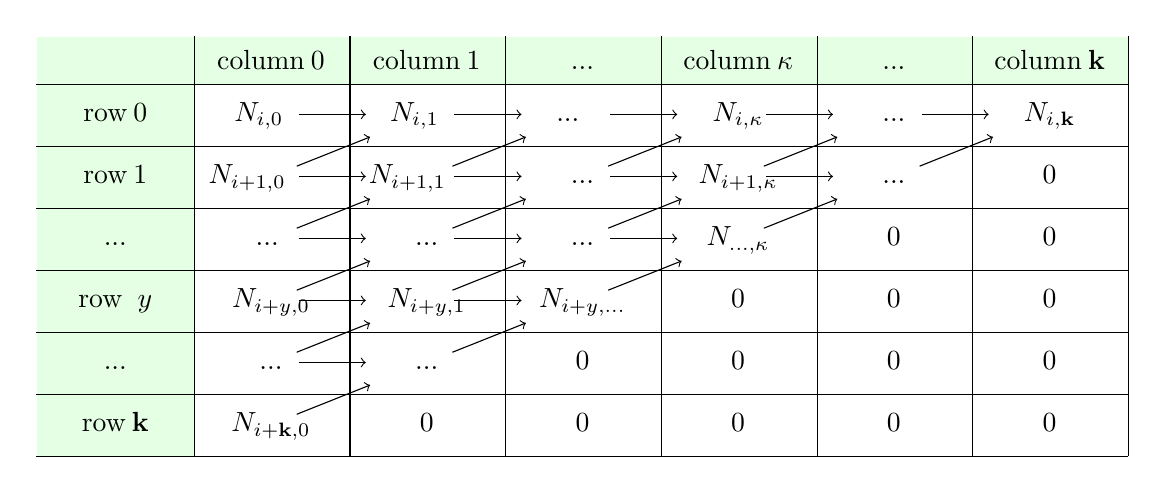
\begin{tikzpicture}
% the matrix entries
\matrix (mat) [table]
{
& column\:0 & column\:1 & ... & column\:$\kappa$ & ... & column\:\textbf{k} \\
row\:0 & $N_{i,0} \;\; $  & $N_{i,1} \;\; $ & ... \;\;  & $ N_{i,\kappa}$ & ... & $ N_{i,\textbf{k}}$\\
row\:1 & $N_{i+1,0}$ \;\;\;\;\; & $N_{i+1,1}$\;\;\;\;\; & ... & $ N_{i+1,\kappa}$ & ... & 0\\
... & ...\; & ... & ... & $N_{...,\kappa}$ & 0 & 0\\
row\: $y$ & $N_{i+y,0}$ & $N_{i+y,1}$ & $N_{i+y,...}$ & 0 & 0 & 0\\
... & ... & ... & 0 & 0 & 0 & 0\\
row\:\textbf{k} & $N_{i+\textbf{k},0}$ & 0 & 0 & 0 & 0 & 0\\
};
% the matrix rules
\foreach \x in {1,...,7}
{
  \draw 
    ([xshift=-.5\pgflinewidth]mat-\x-1.south west) --   
    ([xshift=-.5\pgflinewidth]mat-\x-7.south east);
  }
\foreach \x in {1,...,7}
{
  \draw 
    ([yshift=.5\pgflinewidth]mat-1-\x.north east) -- 
    ([yshift=.5\pgflinewidth]mat-7-\x.south east);
}    
% the arrows
\begin{scope}[shorten >=22pt,shorten <= 10pt]
\draw[->]  (mat-2-2.center) -- (mat-2-3.center);
\draw[->]  (mat-2-3.center) -- (mat-2-4.center);
\draw[->]  (mat-2-4.center) -- (mat-2-5.center);
\draw[->]  (mat-2-5.center) -- (mat-2-6.center);
\draw[->]  (mat-2-6.center) -- (mat-2-7.center);
\draw[->]  (mat-3-2.center) -- (mat-3-3.center);
\draw[->]  (mat-3-3.center) -- (mat-3-4.center);
\draw[->]  (mat-3-4.center) -- (mat-3-5.center);
\draw[->]  (mat-3-5.center) -- (mat-3-6.center);
\draw[->]  (mat-4-2.center) -- (mat-4-3.center);
\draw[->]  (mat-4-3.center) -- (mat-4-4.center);
\draw[->]  (mat-4-4.center) -- (mat-4-5.center);
\draw[->]  (mat-5-2.center) -- (mat-5-3.center);
\draw[->]  (mat-5-3.center) -- (mat-5-4.center);
\draw[->]  (mat-6-2.center) -- (mat-6-3.center);

\draw[->]  (mat-7-2.center) -- (mat-6-3.center);
\draw[->]  (mat-6-2.center) -- (mat-5-3.center);
\draw[->]  (mat-6-3.center) -- (mat-5-4.center);
\draw[->]  (mat-5-2.center) -- (mat-4-3.center);
\draw[->]  (mat-5-3.center) -- (mat-4-4.center);
\draw[->]  (mat-5-4.center) -- (mat-4-5.center);
\draw[->]  (mat-4-2.center) -- (mat-3-3.center);
\draw[->]  (mat-4-3.center) -- (mat-3-4.center);
\draw[->]  (mat-4-4.center) -- (mat-3-5.center);
\draw[->]  (mat-4-5.center) -- (mat-3-6.center);
\draw[->]  (mat-3-2.center) -- (mat-2-3.center);
\draw[->]  (mat-3-3.center) -- (mat-2-4.center);
\draw[->]  (mat-3-4.center) -- (mat-2-5.center);
\draw[->]  (mat-3-5.center) -- (mat-2-6.center);
\draw[->]  (mat-3-6.center) -- (mat-2-7.center);


\end{scope}
\end{tikzpicture}

\begin{equation} \label{right arrow}
    \rightarrow \:\: = \: \times \; \frac{t - t_{i+y}}{t_{i+y+\kappa} - t_{i+y}} \; + 
\end{equation}

\begin{equation} \label{diag arrow}
    \nearrow \:\:  = \times \; \frac{t_{i+y+\kappa+1} - t}{t_{i+y+\kappa+1}-t_{i+y+1}} \; + 
\end{equation}

\hspace{1cm}

OPEN B-SPLINE

\hspace{1cm}

For the \(i^{th}\) basis function at time (t), we have each cell of the table \say{\(N_{t,i}\)} equal to the following.

\begin{equation} \label{eq:table Basis function}
    N_{t,i}[y,\kappa] = \frac{t - t_{i+y}}{t_{i+y+\kappa} - t_{i+y}} N_{t,i}[y,\kappa-1] + \frac{t_{i+y+\kappa+1} - t}{t_{i+y+\kappa+1}-t_{i+y+1}} N_{t,i}[y+1,\kappa-1]
\end{equation}

\begin{equation} \label{eq:table Basis function equation zeros}
      N_{t,i}[y,0] =   \begin{cases} 1, &  \text{if} \quad t_{i+y} \leq t < t_{i+y+1} \\
                            0, & \text{otherwise} \end{cases}
  \end{equation}
  
\hspace{1cm}

CLAMPED B-SPLINE

\hspace{1cm}

For a clamped B-spline, the basis function is evaluated as follows.

\begin{equation} \label{eq:table evaluation clamped}
    N_{t,i}[y,\kappa] = \begin{cases} \quad 0, & \text{if} \quad t_{i+y+k} \leq t_{i+y} \quad \text{\&} \quad t_{i+y+k+1} \leq t_{i+y+1}\\\\
    \frac{t - t_{i+y}}{t_{i+y+\kappa} - t_{i+y}} N_{t,i}[y,\kappa-1], & \text{if} \quad t_{i+y+k} > t_{i+y} \quad \text{\&} \quad t_{i+y+k+1} \leq t_{i+y+1} \\\\
    \frac{t_{i+y+\kappa+1} - t}{t_{i+y+\kappa+1}-t_{i+y+1}} N_{t,i}[y+1,\kappa-1],  & \text{if} \quad t_{i+y+k} \leq t_{i+y} \quad \text{\&} \quad t_{i+y+k+1} > t_{i+y+1}\\\\
    \frac{t - t_{i+y}}{t_{i+y+\kappa} - t_{i+y}} N_{t,i}[y,\kappa-1] \quad + \\ \frac{t_{i+y+\kappa+1} - t}{t_{i+y+\kappa+1}-t_{i+y+1}} N_{t,i}[y+1,\kappa-1], & \text{otherwise}
    \end{cases}
\end{equation}

\begin{equation} \label{eq:table evaluation clamped zeros}
      N_{t,i}[y,0] =   \begin{cases} 1, &  \text{if} \quad t_{i+y} \leq t < t_{i+y+1} \\
      1, &  \text{if} \quad t = t_n = t_{i+y+1} \\
                            0, & \text{otherwise} \end{cases}
  \end{equation}

\subsection{Matrix Method} \label{matrix mehtod}

\subsubsection{Open B-Spline}
    
GENERAL EQUATION - OPEN B-SPLINE

\hspace{1cm}

The matrix equation for an open uniform B-Spline is shown below.
    
    \begin{equation}
        b(t) = \textbf{P}_i M L
    \end{equation}

        where
    
    \begin{equation}
    M \in \mathbb{R}^{\textbf{k}+1 \times \textbf{k}+1}
    \end{equation}
        
    \begin{equation}
        \textbf{P}_i = \begin{bmatrix} P_{i} & P_{i+1} & ... & P_{i+\textbf{k}}\end{bmatrix}
    \end{equation}
    
    \begin{equation}
        L = \begin{bmatrix} \tau^{\textbf{k}} \\ ... \\ \\ \tau^2 \\ \tau \\ 1 \end{bmatrix}
    \end{equation}
    
    \begin{equation}
        \tau = \frac{t-t_j}{\alpha}
    \end{equation}
    
    \begin{equation}
        t_j \leq t < t_{j+1} \quad , \quad i = j-\textbf{k}
    \end{equation}
    
Also note that \(M\) is a matrix of constants, unique for the order of the B-spline. An expanded form of the equation is shown below.

\begin{equation}
    c_0 + c_1 t + c_2 t^2 + ... + c_{\textbf{k}} t^{\textbf{k}} = \begin{bmatrix} P_{i} & P_{i+1} & ... & P_{i+\textbf{k}}\end{bmatrix} M \begin{bmatrix} (\frac{t-t_j}{\alpha})^\textbf{k} \\ \\ ... \\ \\ (\frac{t-t_j}{\alpha})^2 \\ \\ (\frac{t-t_j}{\alpha}) \\ \\ 1 \end{bmatrix}
\end{equation}

LINEAR OPEN B-SPLINES
\hfill \break

    The matrix equation for a uniform linear B-Spline. This following equation applies to both open and clamped linear B-splines.
    
    \begin{equation}
        b(t) = \begin{bmatrix} P_i & P_{i+1} \end{bmatrix} \begin{bmatrix} -1 & 1 \\ 1 & 0
        \end{bmatrix} \begin{bmatrix} \tau \\ 1 \end{bmatrix}
    \end{equation}
    
    for
    
    \begin{equation}
        \tau = \frac{t-t_j}{\alpha}
    \end{equation}
    
    \begin{equation}
        t_j < t < t_{j+1} \quad , \quad i = j-\textbf{k}
    \end{equation}
    
    given
    
    \begin{equation}
    \textbf{P} = \begin{bmatrix} P_0, P_1, ... P_{n-1} \end{bmatrix} \quad \text{,} \quad n \geq 2
    \end{equation}
    
    \begin{equation}
        \textbf{T} = \begin{bmatrix} t_0, t_1, ... t_{m-1} \end{bmatrix} \quad \text{,} \quad m \geq 4
    \end{equation}
  
\hspace{1cm}

OPEN QUADRATIC B-SPLINES
\hfill \break

    The matrix equation for a uniform quadratic B-Spline.
    
    \begin{equation}
        b(t) = \begin{bmatrix} P_i & P_{i+1} & P_{i+2} \end{bmatrix} \frac{1}{2} \begin{bmatrix} 1 & -2 & 1 \\ -2 & 2 & 1 \\ 1 & 0 & 0
        \end{bmatrix} \begin{bmatrix} \tau^2 \\ \tau \\ 1 \end{bmatrix}
    \end{equation}
    
    for
    
    \begin{equation}
        \tau = \frac{t-t_j}{\alpha}
    \end{equation}
    
    \begin{equation}
        t_j < t < t_{j+1} \quad , \quad i = j-\textbf{k}
    \end{equation}
    
    given
    
    \begin{equation}
    \textbf{P} = \begin{bmatrix} P_0, P_1, ... P_{n-1} \end{bmatrix} \quad \text{,} \quad n \geq 3
    \end{equation}
    
    \begin{equation}
        \textbf{T} = \begin{bmatrix} t_0, t_1, ... t_{m-1} \end{bmatrix} \quad \text{,} \quad m \geq 6
    \end{equation}

\hspace{1cm}

OPEN CUBIC B-SPLINES
\hfill \break

    The matrix equation for a uniform quadratic B-Spline.
    
    \begin{equation}
        b(t) = \begin{bmatrix} P_i & P_{i+1} & P_{i+2} & P_{i+3} \end{bmatrix} \frac{1}{12} \begin{bmatrix} -2 & 6 & -6 & 2 \\
                                          6 & -12 & 0 & 8 \\
                                         -6 & 6 & 6 & 2 \\
                                          2 & 0 & 0 & 0 \end{bmatrix} \begin{bmatrix} \tau^3 \\ \tau^2 \\ \tau \\ 1 \end{bmatrix}
    \end{equation}
    
    for
    
    \begin{equation}
        \tau = \frac{t-t_j}{\alpha}
    \end{equation}
    
    \begin{equation}
        t_j < t < t_{j+1} \quad , \quad i = j-\textbf{k}
    \end{equation}
    
    given
    
    \begin{equation}
    \textbf{P} = \begin{bmatrix} P_0, P_1, ... P_{n-1} \end{bmatrix} \quad \text{,} \quad n \geq 4
    \end{equation}
    
    \begin{equation}
        \textbf{T} = \begin{bmatrix} t_0, t_1, ... t_{m-1} \end{bmatrix} \quad \text{,} \quad m \geq 8
    \end{equation}
    
\hspace{1cm}
    
OPEN QUARTIC B-SPLINES
\hfill \break

    The matrix equation for a uniform quartic B-Spline.
    
    \begin{equation}
        b(t) = \begin{bmatrix} P_i & P_{i+1} & P_{i+2} & P_{i+3} & P_{i+4} \end{bmatrix} \frac{1}{24} \begin{bmatrix} 1 & -4  &  6 & -4  & 1 \\
                                                  -4 &  12 & -6 & -12 & 11\\
                                                   6 & -12 & -6 &  12 & 11\\
                                                  -4 &  4  &  6 &  4  & 1 \\
                                                   1 &  0  &  0 &  0  & 0\end{bmatrix} \begin{bmatrix} \tau^4 \\ \tau^3 \\ \tau^2 \\ \tau \\ 1 \end{bmatrix}
    \end{equation}
    
    for
    
    \begin{equation}
        \tau = \frac{t-t_j}{\alpha}
    \end{equation}
    
    \begin{equation}
        t_j < t < t_{j+1} \quad , \quad i = j-\textbf{k}
    \end{equation}
    
    given
    
    \begin{equation}
    \textbf{P} = \begin{bmatrix} P_0, P_1, ... P_{n-1} \end{bmatrix} \quad \text{,} \quad n \geq 5
    \end{equation}
    
    \begin{equation}
        \textbf{T} = \begin{bmatrix} t_0, t_1, ... t_{m-1} \end{bmatrix} \quad \text{,} \quad m \geq 10
    \end{equation}

\hspace{1cm}

OPEN QUINTIC B-SPLINES
\hfill \break

    The matrix equation for a uniform quintic B-Spline.
    
    \begin{equation}
        b(t) = \begin{bmatrix} P_i & P_{i+1} & P_{i+2} & P_{i+3} & P_{i+4} & P_{i+5} \end{bmatrix} \frac{1}{120} \begin{bmatrix} -1  &  5  & -10 &  10  & -5  & 1 \\
                                                     5  & -20 &  20 &  20  & -50 & 26\\
                                                    -10 &  30 &  0  & -60  &  0  & 66\\
                                                     10 & -20 & -20 &  20  &  50 & 26\\
                                                    -5  &  5  &  10 &  10  &  5  & 1\\
                                                     1  &  0  &  0  &  0   &  0  & 0\end{bmatrix} \begin{bmatrix} \tau^5 \\ \tau^4 \\ \tau^3 \\ \tau^2 \\ \tau \\ 1 \end{bmatrix}
    \end{equation}
    
    for
    
    \begin{equation}
        \tau = \frac{t-t_j}{\alpha}
    \end{equation}
    
    \begin{equation}
        t_j < t < t_{j+1} \quad , \quad i = j-\textbf{k}
    \end{equation}
    
    given
    
    \begin{equation}
    \textbf{P} = \begin{bmatrix} P_0, P_1, ... P_{n-1} \end{bmatrix} \quad \text{,} \quad n \geq 6
    \end{equation}
    
    \begin{equation}
        \textbf{T} = \begin{bmatrix} t_0, t_1, ... t_{m-1} \end{bmatrix} \quad \text{,} \quad m \geq 12
    \end{equation}

\subsubsection{Clamped B-spline}

\hspace{1cm}
\noindent GENERAL FORM - CLAMPED UNIFORM B-SPLINES
\hfill \break

\begin{figure}[H]
\begin{center}
\includegraphics[scale=.23]{ClampedMatricesReducedN.png}
\end{center}
\caption{A diagram of the matrices required for a specific number of control points}
\label{Fig:ClampedMatricesWithReducedN}
\end{figure}

For a clamped B-spline, the \(M\) matrix takes on different values depending on the interval it is evaluating. These values depend on the order and number of control points used to define the spline. Figure (\ref{Fig:ClampedMatricesWithReducedN}) shows how many unique matrices (\(q\)) are required to define a B-spline given the order (\textbf{k}) and number of control points (n). We also show the number of knot intervals (\(\mu\)). The total number of matrix definitions (c) that exist for a clamped \(\textbf{k}^{th}\) order spline is equal to \(\textbf{k}^{2}\).

Once we have the correct M matrix for a given interval, we use the same equation as for an open B-Spline.

    \begin{equation}
        b(t) = \textbf{P}_i M L
    \end{equation}

\hspace{1cm}
\noindent CLAMPED QUADRATIC B-SPLINES
\hfill \break

    In Figure \ref{Fig:Clamped 2nd Order}, we show a diagram of the matrices needed to define a clamped B-spline, given a number of control points. With 5 or more control points (n), the total number of unique matrices (\(q\)) needed to define the B-spline is 3. The number of unique matrices (\(q\)) decreases as we decrease the number of control points below 5.
    
\begin{figure}[H]
\begin{center}
\includegraphics[scale=.22]{Clamped2ndOrderMatrixPattern.png}
\end{center}
\caption{Matrix evaluation pattern for clamped 2nd order B-splines}
\label{Fig:Clamped 2nd Order}
\end{figure}

See section \ref{sec: Clamped 2nd order matrices} for the values of these matrices.

\hspace{1cm}

\noindent CLAMPED CUBIC B-SPLINES
\hfill \break

\begin{figure}[H]
\begin{center}
\includegraphics[scale=.24]{Clamped3rdOrderMatrixPattern.png}
\end{center}
\caption{Matrix evaluation pattern for clamped 3rd order B-splines}
\label{Fig:Clamped 3rd Order}
\end{figure}

    In Figure \ref{Fig:Clamped 3rd Order}, we show a diagram of the matrices needed to define a 3rd order clamped B-spline, given a specific number of control points.

See section \ref{sec: Clamped 3rd order matrices} for the values of these matrices.

\hspace{1cm}

\noindent CLAMPED QUARTIC B-SPLINES

\hspace{1cm}

\begin{figure}[H]
\begin{center}
\includegraphics[scale=.37]{Clamped4thOrderMatrixPattern.png}
\end{center}
\caption{Matrix evaluation pattern for clamped 4th order B-splines}
\label{Fig:Clamped 4th Order}
\end{figure}

    In Figure \ref{Fig:Clamped 4th Order}, we show a diagram of the matrices needed to define a 4th order clamped B-spline, given a specific number of control points.

See section \ref{sec: Clamped 4th order matrices} for the values of these matrices.

\hspace{1cm}

\hspace{1cm}

\noindent CLAMPED QUINTIC B-SPLINES
\hfill \break

\hspace{1cm}

\begin{figure}[H]
\begin{center}
\includegraphics[scale=.36]{Clamped5thOrderMatrixPattern.png}
\end{center}
\caption{Matrix evaluation pattern for clamped 5th order B-splines}
\label{Fig:Clamped 5th Order}
\end{figure}

    In Figure \ref{Fig:Clamped 5th Order}, we show a diagram of the matrices needed to define a 4th order clamped B-spline, given a specific number of control points. See section \ref{sec: Clamped 5th order matrices} for the values of these matrices.

\hspace{1cm}

\subsubsection{Rapid Evaluation}

To perform a rapid evaluation for a large data set we can use the matrix method to evaluate the B-spline for a set of time data. Let us define (\(\delta\)) as the resolution for the data set, and (\(\eta\)) as the number of data points per knot interval.

\begin{equation}
    \delta = \frac{1}{\eta-1}
\end{equation}

For a given knot interval, the matrix equation is as follows. 


\begin{equation}
\begin{aligned}
    b(t_i \rightarrow t_{i+1}) &= \textbf{P}_i M \textbf{L}\\
    b(t_i \rightarrow t_{i+1}) &= \begin{bmatrix} P_i, & P_{i+1}, & ... & P_{i+\textbf{k}} \end{bmatrix} M \begin{bmatrix} 0 & \delta^{\textbf{k}} & (2\delta)^{\textbf{k}}& ... & \big((\eta-1) \delta\big)^{\textbf{k}}\\
    & ... & & & ... \\ \\
    0^2 &  \delta^2 & (2\delta)^2 & ... & \big((\eta-1) \delta\big)^2 \\ 
     0 &  \delta & 2\delta & ... & (\eta-1) \delta \\ 
     1 & 1 & 1 & ... & 1 \end{bmatrix}_{\in \mathbb{R}^{\textbf{k}+1 \times \eta}}
\end{aligned}
\end{equation}

where

\begin{equation}
    b(t_j \rightarrow t_{j+1}) \in \mathbb{R}^{d \times \eta}, \quad i = j-\textbf{k}
\end{equation}
    
To calculate the data-set for the whole spline, this must be done for each knot interval.

\section{Evaluating Derivatives}

\subsubsection{Recursive Method}

The derivative at time t for a B-spline is equal to the following.

  \begin{equation} \label{eq:B-Spline derivative equation}
      b'(t) = \sum^{j}_{i=j-k} N'_{i,\textbf{k}}(t) P_i
  \end{equation}
  
  and the \(r^{th}\) derivative is as follows.
  
  \begin{equation} \label{eq:B-Spline rth derivative equation}
      b^{(r)}(t) = \sum^{j}_{i=j-k} N^{(r)}_{i,\textbf{k}}(t) P_i
  \end{equation}

where

\begin{equation}
  t_{j} \leq t \le t_{j+1}
\end{equation}

OPEN B-SPLINE

\hspace{1cm}

Below is the equation for the derivative of a basis function of an open-uniform B-spline.

 \begin{equation} \label{eq:Basis function derivative equation}
 \begin{aligned}
  N_{i,\kappa}'(t) = &
  \frac{t - t_i}{t_{i+\kappa} - t_i} N_{i,\kappa-1}'(t) + \frac{1}{t_{i+\kappa} - t_i} N_{i,\kappa-1}(t) \quad + \\
  & \frac{t_{i+\kappa+1} - t}{t_{i+\kappa+1}-t_{i+1}} N_{i+1 , \kappa-1}'(t) +  \frac{-1}{t_{i+\kappa+1}-t_{i+1}} N_{i+1 , \kappa-1}(t)
  \end{aligned}
  \end{equation}
  
  \begin{equation}
      N_{i,0}' = 0
  \end{equation}

 \hspace{1cm}
 
 The definition for the \(r^{th}\) derivative is as follows.
 
  \begin{equation} \label{eq:Basis function rth derivative equation}
 \begin{aligned}
  N^{(r)}_{i,\kappa}(t) = &
  \frac{t - t_i}{t_{i+\kappa} - t_i} N^{(r)}_{i,\kappa-1}(t) + \frac{1}{t_{i+\kappa} - t_i} N^{(r-1)}_{i,\kappa-1}(t) \quad + \\
  & \frac{t_{i+\kappa+1} - t}{t_{i+\kappa+1}-t_{i+1}} N^{(r)}_{i+1 , \kappa-1}(t) +  \frac{-1}{t_{i+\kappa+1}-t_{i+1}} N^{(r-1)}_{i+1 , \kappa-1}(t)
  \end{aligned}
  \end{equation}
  
  \begin{equation}
      N^{(r)}_{i,0} = 0
  \end{equation}

CLAMPED B-SPLINE

\hspace{1cm}

Below is the equation for the \(r^{th}\) derivative of a basis function of a clamped-uniform B-spline.
 
 \begin{equation} \label{eq:Basis function rth derivative equation clamped}
  N^{(r)}_{i,\kappa}(t) = \begin{dcases} \quad 0, & \text{if} \quad t_{i} \geq t_{i+k} \\ & \text{\&} \quad t_{i+1} \geq t_{i+k+1} \\\\
  \frac{t - t_i}{t_{i+\kappa} - t_i} N^{(r)}_{i,\kappa-1}(t) + \frac{1}{t_{i+\kappa} - t_i} N^{(r-1)}_{i,\kappa-1}(t), & \text{if} \quad t_{i} < t_{i+k} \\ & \text{\&} \quad t_{i+1} \geq t_{i+k+1} \\\\
  \frac{t_{i+\kappa+1} - t}{t_{i+\kappa+1}-t_{i+1}} N^{(r)}_{i+1 , \kappa-1}(t) +  \frac{-1}{t_{i+\kappa+1}-t_{i+1}} N^{(r-1)}_{i+1 , \kappa-1}(t), & \text{if} \quad t_{i} \geq t_{i+k} \\ & \text{\&} \quad t_{i+1} < t_{i+k+1} \\\\
  \frac{t - t_i}{t_{i+\kappa} - t_i} N^{(r)}_{i,\kappa-1}(t) + \frac{1}{t_{i+\kappa} - t_i} N^{(r-1)}_{i,\kappa-1}(t) \quad + \\
  \frac{t_{i+\kappa+1} - t}{t_{i+\kappa+1}-t_{i+1}} N^{(r)}_{i+1 , \kappa-1}(t) +  \frac{-1}{t_{i+\kappa+1}-t_{i+1}} N^{(r-1)}_{i+1 , \kappa-1}(t), & \text{otherwise}
  \end{dcases}
  \end{equation}
  
 \hspace{1cm}
 
 \begin{equation} \label{eq:Basis function equation zeros}
      N_{i,0} =   \begin{cases} 1, &  \text{if } \quad t_i \leq t < t_{i+1} \\
                            1, & \text{if } \quad t_i \leq t = t_{i+1} = t_n \\
                            0, & \text{otherwise} \end{cases}
  \end{equation}
  
  \begin{equation}
      N_{i,0}^{(r)} = 0
  \end{equation}
  
\subsection{Table Method}

The derivative at time t for a B-spline is defined by the following table definition

  \begin{equation} \label{eq:B-Spline derivative equation}
      b'(t) = \sum^{j}_{i=j-k} N'_{t,i}[0,\textbf{k}] P_i
  \end{equation}
  
  and the \(r^th\) derivative is as follows.
  
  \begin{equation} \label{eq:B-Spline rth derivative equation}
      b^{(r)}(t) \sum^{j}_{i=j-k} N_{t,i}[0,\textbf{k},r] P_i
  \end{equation}

where

\begin{equation}
  t_{j} \leq t \le t_{j+1}
\end{equation}

\hspace{1cm}

OPEN B-SPLINE

\hspace{1cm}

For the \(i^{th}\) basis function at time (t) we have two tables, \say{\(N_{t,i}\)} and \say{\(N'_{t,i}\)}. Each cell of table \say{\(N'_{t,i}\)} is equal to the following.

 \begin{equation} \label{eq:Basis function table derivative equation}
 \begin{aligned}
  N'_{t,i}[y,\kappa] = & 
  \frac{t - t_{i+y}}{t_{i+y+\kappa} - t_{i+y}} N'_{t,i}[y,\kappa-1] + \frac{1}{t_{i+y+\kappa} - t_{i+y}} N_{t,i}[y,\kappa-1] \quad + \\\\
   & \frac{t_{i+y+\kappa+1} - t}{t_{i+y+\kappa+1}-t_{i+y+1}} N'_{t,i}[y+1 , \kappa-1] +  \frac{-1}{t_{i+y+\kappa+1}-t_{i+y+1}} N_{t,i}[y+1 , \kappa-1]
 \end{aligned}
  \end{equation}
  
\hspace{1cm}
  
  \begin{equation}
      N'_{t,i}[y,0] = 0
  \end{equation}
  
Refer to equations (\ref{eq:table Basis function}) and (\ref{eq:table Basis function equation zeros}) for the values of table \say{\(N_{t,i}\)}. We also show the basis function equations for the \(r^{th}\) derivative using the table method. Here we have a three dimensional table of size \textbf{k} x \textbf{k} x r+1. See figure \ref{Fig:Derivative Table}.

\begin{figure}[H]
\begin{center}
\includegraphics[scale=.25]{tableDerivatives.png}
\end{center}
\caption{The table that is created when evaluating the \(r^{th}\) derivative of a B-spline}
\label{Fig:Derivative Table}
\end{figure}

 \begin{equation} \label{eq:Basis function table derivative equation}
 \begin{aligned}
  N_{t,i}[y,\kappa, \rho] = & 
  \frac{t - t_{i+y}}{t_{i+y+\kappa} - t_{i+y}} N_{t,i}[y,\kappa-1,\rho] + \frac{1}{t_{i+y+\kappa} - t_{i+y}} N_{t,i}[y,\kappa-1,\rho-1] \quad + \\
   & \frac{t_{i+y+\kappa+1} - t}{t_{i+y+\kappa+1}-t_{i+y+1}} N_{t,i}[y+1 , \kappa-1, \rho] \quad + \\ & \frac{-1}{t_{i+y+\kappa+1}-t_{i+y+1}} N_{t,i}[y+1 , \kappa-1, \rho-1]
 \end{aligned}
  \end{equation}
  
\hspace{1cm}
  
  \begin{equation}
      N_{t,i}[y,0,\rho] = 0
  \end{equation}
  
  where
  
  \begin{equation}
      \rho \geq 1
  \end{equation}
  
 Refer to equations (\ref{eq:table evaluation clamped}) and (\ref{eq:table evaluation clamped zeros}) for the values of \say{\(N_{t,i}\)} when \(\rho\) = 0.
  
 \hspace{1cm}
 
CLAMPED B-SPLINE

 \begin{equation} \label{eq:Basis function table rth derivative equation}
  N_{t,i}[y,\kappa, \rho] = \begin{dcases} \quad 0, & \text{if} \quad t_{i+y+k} \leq t_{i+y} \\ & \text{\&} \quad t_{i+y+k+1} \leq t_{i+y+1} \\\\
  \frac{t - t_{i+y}}{t_{i+y+\kappa} - t_{i+y}} N_{t,i}[y,\kappa-1,\rho] \quad + \\ 
  \frac{1}{t_{i+y+\kappa} - t_{i+y}} N_{t,i}[y,\kappa-1,\rho-1], & \text{if} \quad t_{i+y+k} > t_{i+y} \\ & \text{\&} \quad t_{i+y+k+1} \leq t_{i+y+1}\\\\
  \frac{t_{i+y+\kappa+1} - t}{t_{i+y+\kappa+1}-t_{i+y+1}} N_{t,i}[y+1 , \kappa-1, \rho] \quad + \\  \frac{-1}{t_{i+y+\kappa+1}-t_{i+y+1}} N_{t,i}[y+1 , \kappa-1, \rho-1], & \text{if} \quad t_{i+y+k} \leq t_{i+y} \\ & \text{\&} \quad t_{i+y+k+1} > t_{i+y+1} \\\\
  \frac{t - t_{i+y}}{t_{i+y+\kappa} - t_{i+y}} N_{t,i}[y,\kappa-1,\rho] \quad + \\
  \frac{1}{t_{i+y+\kappa} - t_{i+y}} N_{t,i}[y,\kappa-1,\rho-1] \quad + \\
    \frac{t_{i+y+\kappa+1} - t}{t_{i+y+\kappa+1}-t_{i+y+1}} N_{t,i}[y+1 , \kappa-1, \rho] \quad + \\  \frac{-1}{t_{i+y+\kappa+1}-t_{i+y+1}} N_{t,i}[y+1 , \kappa-1, \rho-1], & \text{otherwise}
 \end{dcases}
  \end{equation}
  
\hspace{1cm}
  
  \begin{equation}
      N_{t,i}[y,0,\rho] = 0
  \end{equation}
  
  where
  
  \begin{equation}
      \rho \geq 1
  \end{equation}
  
\hspace{1cm}

Refer to equations (\ref{eq:table evaluation clamped}) and (\ref{eq:table evaluation clamped zeros}) for the values of \say{\(N_{t,i}\)} when \(\rho\) = 0.

\subsection{Matrix Method}

This section describes how take the \(r^{th}\) derivative of a B-Spline. We start by observing the equation for the matrix evaluation of a B-spline.

\begin{equation}
    b(t) = \begin{bmatrix} P_{i} & P_{i+1} & ... & P_{i+\textbf{k}}\end{bmatrix} M \begin{bmatrix} (\frac{t-t_j}{\alpha})^\textbf{k} \\ \\ ... \\ \\ (\frac{t-t_j}{\alpha})^2 \\ \\ (\frac{t-t_j}{\alpha}) \\ \\ 1 \end{bmatrix}
\end{equation}

If we take the derivative of this we get.

\begin{equation}
    b^{\prime}(t) = \begin{bmatrix} P_{i} & P_{i+1} & ... & P_{i+\textbf{k}}\end{bmatrix} M \begin{bmatrix} \frac{\textbf{k}}{\alpha} (\frac{t-t_j}{\alpha})^\textbf{k-1} \\ \\ ... \\ \\ \frac{2}{\alpha}(\frac{t-t_j}{\alpha}) \\ \\ \frac{1}{\alpha} \\ \\ 0 \end{bmatrix}
\end{equation}

We can also represent the \(r^{th}\) derivative.

\begin{equation} \label{rth derviative spline}
    b^{(r)}(t) = \begin{bmatrix} P_{i} & P_{i+1} & ... & P_{i+\textbf{k}}\end{bmatrix} M \begin{bmatrix}
    \frac{(t-t_j)^{\textbf{k}-r} \textbf{k}!}{ \alpha^{\textbf{k}} (\textbf{k}-r)!} \\ \\ \frac{(t-t_j)^{\textbf{k}-1-r} (\textbf{k}-1)!}{ \alpha^{\textbf{k}-1} (\textbf{k}-1-r)!} \\ \\ 
    ... 
    \\ \\ 
    \frac{(t-t_j)(r+1)!}{\alpha^{r+1} 1! } 
    \\ \\ \frac{r!}{\alpha^r 0!} 
    \\ \\ \textbf{0}_{r \times 1} \end{bmatrix}
\end{equation}

We can rewrite equation (\ref{rth derviative spline}) using \(\tau\).

\begin{equation}
    b^{(r)}(t) = \begin{bmatrix} P_{i} & P_{i+1} & ... & P_{i+\textbf{k}}\end{bmatrix} M \begin{bmatrix} \tau^{\textbf{k}-r} \frac{\textbf{k}!}{(\textbf{k}-r)!} \\\\ 
    \tau^{\textbf{k}-r-1} \frac{(\textbf{k}-1)!}{(\textbf{k}-r-1)!} \\\\
    ... 
    \\\\ 
    \tau^2 \frac{(r+2)!}{2!} \\\\
    \tau \frac{(r+1)!}{1!}
    \\\\  \frac{r!}{0!}
    \\\\ \textbf{0}_{r \times 1} \end{bmatrix} \frac{1}{\alpha^r}
\end{equation}

\begin{equation}
    r \leq \textbf{k}
\end{equation}
    
    \begin{equation}
        \tau = \frac{t-t_j}{\alpha}, \quad t_j \leq t < t_{j+1} \quad , \quad i = j-\textbf{k}
    \end{equation}


Note that the M matrix we use depends on the order, number of control points, and whether we are using an open or clamped B-spline. See section \ref{matrix mehtod} to determine which M matrix to use.

\subsubsection{Rapid Derivative Evaluation}

Recall that (\(\delta\)) is the resolution step for the knot interval, (\(\eta\)) is the number of data points per knot interval. The B-spline evaluation for \(\eta\) points in a knot interval is shown below.

\begin{equation}
\begin{aligned}
    b(t_i \rightarrow t_{i+1}) &= \textbf{P}_i M \textbf{K}\textbf{L}_r\\
    b(t_i \rightarrow t_{i+1}) &= \begin{bmatrix} P_i, & P_{i+1}, & ... & P_{i+\textbf{k}} \end{bmatrix} M \textbf{K} \begin{bmatrix} 0 & \delta^{\textbf{k}-r} & (2\delta)^{\textbf{k}-r}& ... & \big((\eta-1) \delta\big)^{\textbf{k}-r}\\
    & ... & & & ... \\ \\
    0^2 &  \delta^2 & (2\delta)^2 & ... & \big((\eta-1) \delta\big)^2 \\ 
     0 &  \delta & 2\delta & ... & (\eta-1) \delta \\ 
     1 & 1 & 1 & ... & 1 \\
     \textbf{0}_{r \times 1} & \textbf{0}_{r \times 1} & \textbf{0}_{r \times 1} & ... & \textbf{0}_{r \times 1}\end{bmatrix}_{\in \mathbb{R}^{\textbf{k}+1 \times \eta}}
\end{aligned}
\end{equation}

where

\begin{equation}
    \textbf{K} = \frac{1}{\alpha^r}\begin{bmatrix} \frac{\textbf{k}!}{(\textbf{k}-r)!} & & & &  \textbf{0}\\ 
    & ... & & & & 
    \\ 
    & &  \frac{(r+1)!}{1!} & &
    \\  & & & \frac{(r)!}{0!} &
    \\ \textbf{0} &  & & & \textbf{0}_{r \times r} \end{bmatrix}_{\in \mathbb{R}^{\textbf{k}+1 \times \textbf{k}+1}}
\end{equation}

\begin{equation}
    b(t_j \rightarrow t_{j+1}) \in \mathbb{R}^{d \times \eta}, \quad i = j-\textbf{k}
\end{equation}
    
To calculate the the data set for the whole spline derivative, this must be done for each knot interval.

\subsection{Control Point Derivative Method}

We can also evaluate B-spline derivatives using the control point derivatives.

\begin{equation}
    b(t)^{(r)} = \sum^{j}_{i=j-k+r} N_{i,\textbf{k}-r}(t) P_i^{(r)}
\end{equation}
  
 or 
 
   \begin{equation}
    b(t)^{(r)} = \sum^{j}_{i=j-k+r} N_{t,i}[0,\textbf{k}-r] P_i^{(r)}
\end{equation}

where 

\begin{equation}
  t_{j} \leq t \le t_{j+1}
\end{equation}
  
  With the corresponding knot vector \(T^{(r)}\). See equation (\ref{eq:T^r}) for the definition of \(T^{(r)}\), and equations (\ref{rth open control point derivative}) and (\ref{rth clamped control point derivative}) for the definition of \(P_i^{(r)}\). We can also use the matrix representation.

   \begin{equation}
        b(t)^{(r)} = \textbf{P}_i^{(r)}  M_{\textbf{k}-r} L
    \end{equation}

        where
        
    \begin{equation}
        \textbf{P}_i^{(r)} = \begin{bmatrix} P_{i}^{(r)} & P_{i+1}^{(r)} & ... & P_{i+\textbf{k}-r}^{(r)}\end{bmatrix}
    \end{equation}
    
    \begin{equation}
        L = \begin{bmatrix} \tau^{\textbf{k}-r} \\ ... \\ \\ \tau^2 \\ \tau \\ 1 \end{bmatrix}
    \end{equation}
    
    \begin{equation}
        \tau = \frac{t-t_j}{\alpha}
    \end{equation}
    
    \begin{equation}
        t_j \leq t < t_{j+1} \quad , \quad i = j-\textbf{k}+r
    \end{equation}
    
And \(M_{\textbf{k}-r}\) is the matrix corresponding to a \(\textbf{k}-r\) order B-spline. 

  

\section{Curvature and Shape}

\subsection{Curvature}

The curvature of a function at a specific point is defined by the circle that best approximates the shape of the curve at that point. It is formally defined by the inverse radius of the circle. See figure \ref{Fig:Curvature}.

\begin{figure}[H]
\begin{center}
\includegraphics[scale=.2]{Curvature.png}
\end{center}
\caption{Curvature defined by the oscillating circle}
\label{Fig:Curvature}
\end{figure}

Curvature of a spline can be evaluated by the following equation.

\begin{equation} \label{curvature}
    C = \frac{||b(t)' \times b(t)''||} {||b(t)'||^3}
\end{equation}

where \(b(t)'\) and \(b(t)''\) is the first and second derivative respectively. For a two dimensional spline this expands to the following equation.

\begin{equation}
    C = \frac{x'y'' - y'x''}{(x'^2 + y'^2)^{3/2}}
\end{equation}

We also show the three dimensional expansion for curvature.

\begin{equation}
    C = \frac{\sqrt{(x'y'' - y'x'')^2 + (z'x'' - x'z'')^2 + (y'z'' - z'y'')^2}}{(x'^2 + y'^2 + z'^2)^{3/2}}
\end{equation}

Figure \ref{Fig:SplineCurvature} shows the plotted curvature of a fifth order B-spline in 2 dimensions. 

\begin{figure}[H]
\begin{center}
\includegraphics[scale=.23]{SplineCurvature.png}
\end{center}
\caption{Curvature of a fifth order B-spline}
\label{Fig:SplineCurvature}
\end{figure}

If we want to plot the curvature for a single dimension, we treat time as a second dimension of the spline and end up with the following.

\begin{equation}
    C(t) = \frac{||(1,x') \times (0,x'')||}{||(1,x')||^{3}} 
\end{equation}

or

\begin{equation}
    C(t) = \frac{x''}{(x'^2 + 1)^{3/2}} 
\end{equation}

\subsection{Angular Rate}

Here we refer to the angular rate of the tangent vector of the path as it progresses along the trajectory. Angular rate is defined by the tangent velocity and radius of the oscillating circle that the path is approximating. See figure \ref{Fig:AngularRate.png}.

\begin{figure}[H]
\centering
\includegraphics[scale=.12]{AngularRate.png}
\caption{Angular Rate along a path}
\label{Fig:AngularRate.png}
\end{figure}

\begin{equation}
    \omega = \frac{\nu}{R} = \nu C
\end{equation}

Using the curvature equation we get the following equation for the angular rate.
\begin{equation}
    \omega(t) = \frac{||b(t)' \times b(t)''||}{||b(t)'||^2} = \frac{||\nu \times a||}{||\nu||^2}
\end{equation}

\subsection{Centripetal Acceleration}

The centripetal acceleration is the portion of acceleration that is perpendicular to the velocity vector. See figure \ref{Centripetal_Acceleration}.

\begin{figure}[H]
\centering
\includegraphics[scale=.22]{CentripetalAcceleration.png}
\caption{Centripetal Acceleration}
\label{Centripetal_Acceleration}
\end{figure}

\begin{equation} \label{eq:Centripetal Physics}
    a_p = \frac{\nu^2}{R} = \nu^2 C
\end{equation}

We can derive the equation for centripetal acceleration with equations (\ref{curvature}) and (\ref{eq:Centripetal Physics}).

\begin{equation}
    a_p = \frac{||b(t)' \times b(t)''||}{||b(t)'||} = \frac{||\nu \times a||}{||\nu||}
\end{equation}

\section{Bezier Curves}

This section describes Bezier curves and their relation to B-spline curves.

\subsection{Nomenclature}

\begin{itemize}
  \item[] B(t) = Bezier curve
  \item[] \textbf{k} = order or degree of the curve
  \item[] \(n_B =\) number of Bezier control points.
  \item[] \(\boldsymbol{\beta}\) = set of Bezier control points
  \item[] \(\beta_i = i^{th}\) Bezier control point.
  \item[] \(\rho_{i , \textbf{k}}\) = \(i^{th}\) Bernstein basis polynomial of a \textbf{k} degree Bezier curve.
  \item[] \(\alpha\) = scale factor that determines length of the time interval
  \item[] \(t_0\) = start time of the Bezier curve
\end{itemize}

\subsection{Definition}

A Bezier curve is a parametric curve or polynomial of degree \textbf{k}, that is defined between the interval \([t_0, t_0 + \alpha]\). A set of discrete control points \(\boldsymbol{\beta}\) shapes the curve. See Figure \ref{Fig:BezierCurves}.

\begin{figure}[H]
\begin{center}
\includegraphics[scale=.3]{BezierCurves.png}
\end{center}
\caption{Bezier Curves of order three through five.}
\label{Fig:BezierCurves}
\end{figure}

The Bernstein formula is shown below.

\begin{equation}
    B(t) = \sum_{i=0}^{\textbf{k}}\beta_i \;\rho_{i,\textbf{k}}(t)
\end{equation}

for

\begin{equation}
    t_0 \leq t \leq (t_0 + \alpha)
\end{equation}

\begin{equation}
    \boldsymbol{\beta} = [\beta_0, \beta_i, ... \beta_{\textbf{k}}]
\end{equation}

\hspace{1cm}

The Bernstein basis polynomial is defined below.

\begin{equation}
    \rho_{i,\textbf{k}}(t) = \binom{\textbf{k}}{i}(1 - \tau)^{\textbf{k}-i}\;\tau^i
\end{equation}

where

\begin{equation}
    \tau = \frac{t-t_0}{\alpha}
\end{equation}

The term \(\binom{\kappa}{i}\) is known as a binomial coefficient. Also note that the order of the Bezier Curve is determined by the number of control points. 

\begin{equation}
    n_B = \textbf{k} + 1
\end{equation}

\subsection{Evaluation}

\subsubsection{De Casteljau's Algorithm}
 
 The most common way to evaluate a Bezier curve is using De Casteljau's Algorithm, where we have the following recurrence relation. 
 
 \begin{equation}
     B(t) = \beta_0^{(\textbf{k})}
 \end{equation}
 
 \begin{equation}
     \beta_i^{(j)} = (1-\tau)\beta_i^{(j-1)} + \tau\beta_{i+1}^{(j-1)}
 \end{equation}
 
 \begin{equation}
     \beta_i^{(0)} = \beta_i
 \end{equation}

This approach is usually slower than the direct approach, but is more numerically stable.

\subsubsection{Matrix Approach} \label{Bezier Curve Matrix Approach}
    Evaluating a Bezier curve using matrices has the same form as a B-spline. The matrix equation for a Bezier curve is shown.
    
    \begin{equation}
        B(t) = \boldsymbol{\beta} M_B L
    \end{equation}

        where
    
    \begin{equation}
    M_B \in \mathbb{R}^{\textbf{k}+1 \times \textbf{k}+1}
    \end{equation}
        
    \begin{equation}
        \boldsymbol{\beta} = \begin{bmatrix} \beta_{0} & \beta_{1} & ... & \beta_{\textbf{k}}\end{bmatrix}
    \end{equation}
    
    \begin{equation}
        L = \begin{bmatrix} \tau^{\textbf{k}} \\ ... \\ \\ \tau^2 \\ \tau \\ 1 \end{bmatrix}
    \end{equation}
    
    and
    
    \begin{equation}
        \tau = \frac{t-t_0}{\alpha}, \quad t_0 \leq t < (t_0 + \alpha)
    \end{equation}
    
The M matrices for a 1st through 5th order Bezier curve.

    \begin{flalign*}
            \begin{bmatrix} -1 & 1 \\
                                        1 & 0 \end{bmatrix} \quad \text{if} \quad \textbf{k} = 1 \\\\
            \frac{1}{2}\begin{bmatrix} 2 & -4 & 2 \\
                                        -4 & 4 & 0 \\
                                        2 & 0 & 0 \end{bmatrix} \quad \text{if} \quad \textbf{k} = 2 \\\\
            \frac{1}{12} \begin{bmatrix} -12 & 36 & -36 & 12 \\
                                        36 & -72 & 36 & 0 \\
                                        -36 & 36 & 0 & 0 \\
                                        12 & 0 & 0 & 0\end{bmatrix} \quad \text{if} \quad  \textbf{k} = 3 \\\\
            \begin{bmatrix}1  &  -4 & 6   &-4 & 1\\
                      -4 &  12 & -12 & 4 & 0\\
                      6 & -12 &  6  & 0 & 0\\
                      -4 &  4  & 0   & 0 & 0\\
                     1   &   0 &   0 & 0 & 0\end{bmatrix}  \quad \text{if} \quad \textbf{k} = 4 \\\\
            \begin{bmatrix} -1& 5& -10& 10& -5& 1\\
                      5& -20 & 30 & -20& 5& 0\\
                      -10& 30 & -30& 10& 0 & 0\\
                      10& -20& 10& 0 & 0 & 0\\
                      -5& 5 & 0 & 0 & 0& 0\\
                      1& 0 & 0 & 0 & 0 & 0\end{bmatrix} \quad \text{if} \quad \textbf{k} = 5
        \end{flalign*}
    
\subsection{Relation to B-splines}

A B-spline is composed of n-\textbf{k} Bezier curves. In other words, a B-spline can be thought of as a piece wise set of Bezier curves where the endpoints connecting each curve is differentiable up to the \((k-1)^{th}\) derivative. 

Each set of control points \(\textbf{P}_i\) that define a knot interval can be transformed into a set of Bezier control points \(\boldsymbol{\beta}\) that define the same curve. Figure \ref{Fig:BsplineToBezier} shows a depiction of a set of open uniform B-spline control points converted to Bezier control points.

\begin{figure}[H]
\begin{center}
\includegraphics[scale=.3]{BsplineToBezier.png}
\end{center}
\caption{Set of B-spline control points converted to Bezier control points.}
\label{Fig:BsplineToBezier}
\end{figure}

\subsubsection{Converting to Open B-splines}

The equation to transform a set of Bezier control points to B-spline control points are as follows.

\begin{equation}
    \boldsymbol{\beta} F = \textbf{P}_i
\end{equation}

or

\begin{equation}
    [\beta_0, \beta_1, ... \beta_{\textbf{k}}] F = [P_i, P_{i+1}, ... P_{i+\textbf{k}}]
\end{equation}

Where F is a transformation matrix. Listed below are the values for F to convert Bezier control points to control points of an Open Uniform B-spline for curves of order 1-5.

    \begin{flalign*}
            \begin{bmatrix} 1 & 0 \\
0 & 1 \end{bmatrix} \quad \text{if} \quad \textbf{k} = 1 \\\\
            \begin{bmatrix} 2& 0& 0 \\
-1& 1& -1 \\
0& 0& 2 \end{bmatrix} \quad \text{if} \quad \textbf{k} = 2 \\\\
            \begin{bmatrix} 6 & 0 & 0 & 0 \\
-7 & 2 & -1 & 2 \\
2 & -1 & 2 & -7 \\
0 & 0 & 0 & 6\end{bmatrix} \quad \text{if} \quad  \textbf{k} = 3 \\\\
            \begin{bmatrix}   24& 0& 0& 0& 0\\
  -46& 6& -2& 2& -6\\
   29& -7& 5& -7& 29\\
   -6& 2& -2& 6& -46\\
   0& 0& 0& 0& 24\end{bmatrix}  \quad \text{if} \quad \textbf{k} = 4 \\\\
            \begin{bmatrix} 120&     0&     0 &   0 &   0  &  0 \\
 -326  & 24  & -6 &   4 &  -6 &  24\\
  329 & -46 &  19 & -16 &  29 & -146\\
 -146 &  29 & -16 &  19 & -46 & 329\\
   24 &  -6  &  4 &  -6 &  24 & -326\\
   0 &   0  & 0  & 0 &  0 & 120\end{bmatrix} \quad \text{if} \quad \textbf{k} = 5
        \end{flalign*}

\subsubsection{Converting to Clamped B-splines}

Notice the matrices in section \ref{sec:Clamped B-Spline Matrices} of the Appendix. The matrices under the condition where n = (\textbf{k} + 1) are the same matrices that are used to evaluate Bezier curves in section \ref{Bezier Curve Matrix Approach}. We find that under these conditions, the control points for a Clamped B-spline and for a Bezier Curve are the same.

However, when the number of control points increase for a B-spline, a conversion matrix F is needed for each unique M matrix of the Clamped B-spline. 

\section{Appendix}

    \subsection{Clamped B-Spline Matrices} \label{sec:Clamped B-Spline Matrices}
    
    In these sections \(i_t\) is index for the preceding knot point of the current B-spline interval.
    
    \subsubsection{2nd Order} \label{sec: Clamped 2nd order matrices}
    
        \begin{equation}
        M = \begin{dcases} 
            \frac{1}{2}\begin{bmatrix} 2 & -4 & 2 \\
                                        -4 & 4 & 0 \\
                                        2 & 0 & 0 \end{bmatrix} \quad \textbf{if} \quad n = 3 \\\\
            \frac{1}{2} \begin{bmatrix} 2 & -4 & 2 \\
                                        -3 & 4 & 0 \\
                                        1 & 0 & 0 \end{bmatrix} \quad \textbf{if} \quad n \geq 4  \quad \textbf{and} \quad i_t = 2 \\\\
            \frac{1}{2} \begin{bmatrix} 1 & -2 & 1 \\
                                        -3 & 2 & 1 \\
                                        2 & 0 & 0 \end{bmatrix} \quad \textbf{if} \quad n \geq 4  \quad \textbf{and} \quad i_t = n-1 \\\\
            \frac{1}{2} \begin{bmatrix} 1 & -2 & 1 \\
                                        -2 & 2 & 1 \\
                                        1 & 0 & 0 \end{bmatrix} \quad \textbf{otherwise}
        \end{dcases}
    \end{equation}
    
    given
    
    \begin{equation}
        \quad n \geq 3 \quad \text{and} \quad m \geq 6
    \end{equation}
    
    \subsubsection{3rd Order} \label{sec: Clamped 3rd order matrices}
    
  \begin{equation}
        M = \begin{dcases} 
            \frac{1}{12}\begin{bmatrix} -12 &  36 & -36 & 12 \\
                                         36 & -72 & 36 & 0 \\
                                        -36 &  36 & 0 & 0 \\
                                         12 &  0  & 0 & 0 \end{bmatrix} \quad \textbf{if} \quad n = 4 \\\\
            \frac{1}{12}\begin{bmatrix} -12 &  36 & -36 & 12 \\
                                         21 & -54 &  36 & 0 \\
                                        -12 &  18 &  0  & 0 \\
                                          3 &  0  &  0  & 0 \end{bmatrix} \quad \textbf{if} \quad n = 5 \quad \textbf{and} \quad i_t = 3 \\\\
            \frac{1}{12}\begin{bmatrix} -3  &  9   & -9 & 3 \\
                                         12 & -18  &  0 & 6 \\
                                        -21 &  9   &  9 & 3 \\
                                         12 &  0   &  0 & 0 \end{bmatrix} \quad \textbf{if} \quad n = 5 \quad \textbf{and} \quad i_t = 4 \\\\
            \frac{1}{12}\begin{bmatrix} -12 &  36 & -36 & 12 \\
                                         21 & -54 &  36 & 0\\
                                        -11 &  18 &  0  & 0\\
                                         2  &  0  &  0  & 0 \end{bmatrix} \quad \textbf{if} \quad n \geq 6 \quad \textbf{and} \quad i_t = 3 \\\\
            \frac{1}{12}\begin{bmatrix} -3 & 9 & -9 & 3 \\
                                         7 & -15 & 3 & 7\\
                                        -7 & 6 & 6 & 2\\
                                         3 & 0 & 0 & 0 \end{bmatrix} \quad \textbf{if} \quad n \geq 6 \quad \textbf{and} \quad i_t = 4 \quad \textbf{and} \quad t_{4} = t_{n-2}  \\\\
            \frac{1}{12}\begin{bmatrix} -3 &  9 & -9 & 3 \\
                                         7 & -15 &  3 & 7\\
                                        -6 &  6 & 6 & 2\\
                                         2 &  0 &  0 & 0 \end{bmatrix} \quad \textbf{if} \quad n \geq 6 \quad \textbf{and} \quad i_t = 4 \quad \textbf{and} \quad t_{4} < t_{n-2}  \\\\
            \frac{1}{12}\begin{bmatrix} -2 &  6 & -6 & 2 \\
                                         6 & -12 &  0 & 8\\
                                        -7 &  6 & 6 & 2\\
                                         3 &  0 &  0 & 0 \end{bmatrix} \quad \textbf{if} \quad n \geq 6 \quad \textbf{and} \quad i_t = n-2 \quad \textbf{and} \quad t_{4} < t_{n-2}  \\\\
            \frac{1}{12}\begin{bmatrix} -2 &  6 & -6 & 2 \\
                                         11 & -15  & -3 &  7\\
                                        -21&  9   &  9 &  3\\
                                         12 &  0   &  0 &  0 \end{bmatrix} \quad \textbf{if} \quad n \geq 6 \quad \textbf{and} \quad i_t = n-1 \\\\
            \frac{1}{12}\begin{bmatrix} -2 &  6 & -6 & 2\\
                                         6 & -12 &  0 & 8\\
                                        -6 &  6 &  6 & 2\\
                                         2 &  0 &  0 & 0\end{bmatrix} \quad \textbf{otherwise}
        \end{dcases}
    \end{equation}

    given
    
    \begin{equation}
        n \geq 4 \quad m \geq 8
    \end{equation}
    
    \subsubsection{4th Order} \label{sec: Clamped 4th order matrices}

\begin{flalign}
    M &= &&
\end{flalign}

\begin{flalign*}
        & \begin{bmatrix}1  &  -4 & 6   &-4 & 1\\
                      -4 &  12 & -12 & 4 & 0\\
                      6 & -12 &  6  & 0 & 0\\
                      -4 &  4  & 0   & 0 & 0\\
                     1   &   0 &   0 & 0 & 0\end{bmatrix} \quad \textbf{if} \quad n = 5 \\\\
            & \frac{1}{8}\begin{bmatrix}8  & -32& 48 & -32& 8\\
                        -15& 56 & -72& 32 & 0\\
                        11 & -32& 24 & 0 & 0\\
                        -5 & 8 & 0 & 0 & 0\\
                        1 & 0 & 0 & 0 & 0\end{bmatrix} \quad \textbf{if} \quad n == 6 \quad \textbf{and} \quad i_t = 4 \\\\
            & \frac{1}{8}\begin{bmatrix}1  & -4& 6 & -4& 1\\
                        -5& 12 & -6& -4 & 3\\
                        11 & -12& -6 & 4 & 3\\
                        -15 & 4 & 6 & 4 & 1\\
                        8 & 0 & 0 & 0 & 0\end{bmatrix} \quad \textbf{if} \quad n == 6 \quad \textbf{and} \quad i_t = 5 \\\\
            & \frac{1}{72}\begin{bmatrix}72& -288& 432& -288& 72\\
                        -135& 504& -648& 288& 0\\
                        85& -264& 216& 0 & 0\\
                        -26& 48& 0& 0 &0\\
                        4& 0 & 0 & 0& 0\end{bmatrix} \quad \textbf{if} \quad n == 7 \quad \textbf{and} \quad i_t = 4 \\\\
            & \frac{1}{72}\begin{bmatrix}9& -36& 54& -36& 9\\
                        -23& 76& -66& -20& 37\\
                        28& -56& -12& 40 & 22\\
                        -23& 16& 24& 16 &4\\
                        9& 0 & 0 & 0& 0\end{bmatrix} \quad \textbf{if} \quad n == 7 \quad \textbf{and} \quad i_t = 5 \\\\
            & \frac{1}{72}\begin{bmatrix}4 & -16 & 24 & -16 & 4\\
                          -26 & 56 & -12 & -40 & 22\\
                          85 & -76 & -66 & 20 & 37\\
                          -135 & 36 & 54 & 36 & 9\\
                          72 & 0 & 0 & 0 & 0\end{bmatrix} \quad \textbf{if} \quad n == 7 \quad \textbf{and} \quad i_t = 6 \\\\
            & \frac{1}{72}\begin{bmatrix}72& -288& 432& -288& 72\\
                        -135& 504& -648& 288& 0\\
                        85& -264& 216& 0 & 0\\
                        -25& 48& 0& 0 &0\\
                        3& 0 & 0 & 0& 0\end{bmatrix} \quad \textbf{if} \quad n \geq 8 \quad \textbf{and} \quad i_t = 4 \\\\
                & \frac{1}{72}\begin{bmatrix}9 & -36 & 54 & -36& 9\\
                            -23& 76& -66& -20& 37\\
                            23& -52& -6& 44& 23\\
                            -13& 12& 18& 12& 3\\
                            4& 0 & 0 & 0& 0\end{bmatrix} \quad \textbf{if} \quad \geq 8 \quad \textbf{and} \quad i_t = 5 \quad \textbf{and} \quad t_{5} = t_{n-3} \\\\
                & \frac{1}{72}\begin{bmatrix}9 & -36 & 54 & -36& 9\\
                            -23& 76& -66& -20& 37\\
                            23& -52& -6& 44& 23\\
                            -12& 12& 18& 12& 3\\
                            3& 0 & 0 & 0& 0\end{bmatrix} \quad \textbf{if} \quad \geq 8 \quad \textbf{and} \quad i_t = 5 \quad \textbf{and} \quad t_{5} < t_{n-3} \\\\
                & \frac{1}{72}\begin{bmatrix}4& -16& 24& -16& 4\\
                            -13& 40& -24& -32& 32\\
                            23& -40& -24& 32& 32\\
                            -23& 16& 24& 16& 4\\
                            9& 0 & 0& 0 & 0\end{bmatrix} \quad \textbf{if} \quad \geq 8 \quad \textbf{and} \quad i_t = 6 \quad \textbf{and} \quad t_{6} = t_{n-2} \\\\
                & \frac{1}{72}\begin{bmatrix}4&-16&24&-16&4\\
                              -13&40&-24&-32&32\\
                              18&-36&-18&36&33\\
                              -13&12&18&12&3\\
                              4&0&0&0&0\end{bmatrix} \quad \textbf{if} \quad \geq 8 \quad \textbf{and} \quad i_t = 6 \quad \textbf{and} \quad t_{6} = t_{n-3} \\\\
                & \frac{1}{72}\begin{bmatrix}4&-16&24&-16&4\\
                              -13&40&-24&-32&32\\
                              18&-36&-18&36&33\\
                              -12&12&18&12&3\\
                              3&0&0&0&0\end{bmatrix} \quad \textbf{if} \quad \geq 8 \quad \textbf{and} \quad i_t = 6 \quad \textbf{and} \quad t_{6} < t_{n-3} \\\\
                & \frac{1}{72}\begin{bmatrix}3& -12& 18& -12& 3\\
                              -12& 36& -18& -36& 33\\
                              18& -36& -18& 36& 33\\
                              -13& 12& 18& 12& 3\\
                              4& 0 & 0 & 0 & 0\end{bmatrix} \quad \textbf{if} \quad \geq 8 \quad \textbf{and} \quad i_t = n-3 \quad \textbf{and} \quad t_{6} < t_{n-3} \\\\
                & \frac{1}{72}\begin{bmatrix}3& -12& 18& -12& 3\\
                            -12& 36& -18& -36& 33\\
                            23& -40& -24& 32& 32\\
                            -23& 16& 24& 16& 4\\
                            9& 0 & 0& 0 & 0\end{bmatrix} \quad \textbf{if} \quad \geq 8 \quad \textbf{and} \quad i_t = n-2 \quad \textbf{and} \quad t_{6} < t_{n-2} \\\\
                & \frac{1}{72}\begin{bmatrix}   3& -12& 18& -12& 3\\
                          -25& 52& -6& -44& 23\\
                          85& -76& -66& 20& 37\\
                          -135& 36& 54& 36& 9\\
                          72& 0 & 0 & 0 &0\end{bmatrix} \quad \textbf{if} \quad \geq 8 \quad \textbf{and} \quad i_t = n-1 \\\\
                & \frac{1}{24}\begin{bmatrix}   3& -12& 18& -12& 3\\
                                              -25& 52& -6& -44& 23\\
                                                85& -76& -66& 20& 37\\
                                             -135& 36& 54& 36& 9\\
                                                72& 0 & 0 & 0 &0\end{bmatrix} \quad \textbf{otherwise} \\\\
\end{flalign*}

given
    
    \begin{equation}
        n \geq 5\quad \text{and} \quad m \geq 10
    \end{equation}
    
    \subsubsection{5th Order} \label{sec: Clamped 5th order matrices}
    

\begin{flalign}
    M &= &&
\end{flalign}

\begin{flalign*}
        & \begin{bmatrix} -1& 5& -10& 10& -5& 1\\
                      5& -20 & 30 & -20& 5& 0\\
                      -10& 30 & -30& 10& 0 & 0\\
                      10& -20& 10& 0 & 0 & 0\\
                      -5& 5 & 0 & 0 & 0& 0\\
                      1& 0 & 0 & 0 & 0 & 0\end{bmatrix} \quad \textbf{if} \quad n = 6 \\\\
            & \frac{1}{16}\begin{bmatrix}-16& 80& -160& 160& -80& 16\\
                      31& -150 & 280 & -240& 80& 0\\
                      -26& 110 & -160& 80& 0 & 0\\
                      16& -50& 40& 0 & 0 & 0\\
                      -6& 10 & 0 & 0 & 0& 0\\
                      1& 0 & 0 & 0 & 0 & 0\end{bmatrix} \quad \textbf{if} \quad n = 7 \quad \text{and} \quad i_t = 5 \\\\
            & \frac{1}{16}\begin{bmatrix}-1& 5& -10& 10& -5& 1\\
                      6& -20 & 20 & 0& -10& 4\\
                      -16& 30 & 0& -20& 0 & 6\\
                      26& -20& -20& 0 & 10 & 4\\
                      -31& 5 & 10 & 10 & 5& 1\\
                      16& 0 & 0 & 0 & 0 & 0\end{bmatrix} \quad \textbf{if} \quad n = 7 \quad \text{and} \quad i_t = 6 \\\\
            & \frac{1}{432}\begin{bmatrix}-432& 2160& -4320& 4320& -2160& 432\\
                          837& -4050& 7560& -6480& 2160& 0\\
                          -575& 2550& -3960& 2160& 0 & 0\\
                          222& -780& 720& 0 & 0& 0\\
                          -60& 120& 0 & 0 & 0 & 0\\
                          8& 0 & 0 & 0 & 0 & 0\end{bmatrix} \quad \textbf{if} \quad n = 8 \quad \text{and} \quad i_t = 5 \\\\
            & \frac{1}{432}\begin{bmatrix}-27& 135& -270& 270& -135& 27\\
                          73& -325& 490& -170& -235& 175\\
                          -102& 330& -180& -300& 150 & 162\\
                          102& -180& -120& 120 & 180& 60\\
                          -73& 40& 80 & 80 & 40 & 8\\
                          27& 0 & 0 & 0 & 0 & 0\end{bmatrix} \quad \textbf{if} \quad n = 8 \quad \text{and} \quad i_t = 6 \\\\
            & \frac{1}{432}\begin{bmatrix}-8& 40& -80& 80& -40& 8\\
                          60& -180& 120& 120& -180& 60\\
                          -222& 330& 180& -300& -150& 162\\
                          575& -325& -490& -170& 235& 175\\
                          -837& 135& 270& 270& 135& 27\\
                          432& 0 & 0 & 0 & 0& 0\end{bmatrix} \quad \textbf{if} \quad n = 8 \quad \text{and} \quad i_t = 7 \\\\
            & \frac{1}{864}\begin{bmatrix}-864& 4320& -8640& 8640& -4320& 864\\
                          1674& -8100& 15120& -12960& 4320& 0\\
                          -1150& 5100& -7920& 4320& 0& 0\\
                          415& -1500& 1440& 0 & 0 & 0\\
                          -84& 180& 0 & 0 & 0 & 0\\
                          9 & 0 & 0 & 0 & 0 & 0\end{bmatrix} \quad \textbf{if} \quad n = 9 \quad \text{and} \quad i_t = 5 \\\\
            & \frac{1}{864}\begin{bmatrix}-54& 270& -540& 540& -270& 54\\
                          146& -650& 980& -340& -470& 350\\
                          -161& 575& -410& -530& 395& 355\\
                          108& -240& -120& 240& 300& 96\\
                          -55& 45& 90& 90& 45& 9\\
                          16& 0 & 0 & 0 & 0& 0\end{bmatrix} \quad \textbf{if} \quad n = 9 \quad \text{and} \quad i_t = 6 \\\\
            & \frac{1}{864}\begin{bmatrix}-16& 80& -160& 160& -80& 16\\
                          55& -230& 280& 80& -400& 224\\
                          -108& 300& 0 & -480& 0& 384\\
                          161& -230& -280& 80& 400& 224\\
                          -146& 80& 160& 160& 80& 16\\
                          54& 0 & 0 & 0 & 0 & 0\end{bmatrix} \quad \textbf{if} \quad n = 9 \quad \text{and} \quad i_t = 7 \\\\
            & \frac{1}{864}\begin{bmatrix}-9& 45& -90& 90& -45& 9\\
                          84& -240& 120& 240& -300& 96\\
                          -415& 575& 410& -530& -395& 355\\
                          1150& -650& -980& -340& 470& 350\\
                          -1674& 270& 540& 540& 270& 54\\
                          864& 0 & 0 & 0 & 0 & 0\end{bmatrix} \quad \textbf{if} \quad n = 9 \quad \text{and} \quad i_t = 8 \\\\
            & \frac{1}{4320}\begin{bmatrix}-4320& 21600& -43200& 43200& -21600& 4320\\
                          8370& -40500& 75600& -64800& 21600& 0\\
                          -5750& 25500& -39600& 21600 & 0& 0\\
                          2075& -7500& 7200& 0 & 0 & 0\\
                          -411& 900& 0 & 0 & 0 & 0\\
                          36& 0 & 0 & 0 & 0 & 0\end{bmatrix} \quad \textbf{if} \quad n \geq 10 \quad \text{and} \quad i_t = 5 \\\\
                & \frac{1}{4320}\begin{bmatrix}-270& 1350& -2700& 2700& -1350& 270\\
                              730& -3250& 4900& -1700& -2350& 1750\\
                              -805& 2875& -2050& -2650& 1975& 1775\\
                              489& -1155& -510& 1290& 1545& 489\\
                              -189& 180& 360& 360& 180& 36\\
                              45& 0 & 0& 0& 0& 0\end{bmatrix} \quad \textbf{if} \quad n \geq 10 \quad \text{and} \quad i_t = 6  \quad \text{and} t_{6} = t_{n-4} \\\\
                & \frac{1}{4320}\begin{bmatrix}-270& 1350& -2700& 2700& -1350& 270\\
                              730& -3250& 4900& -1700& -2350& 1750\\
                              -805& 2875& -2050& -2650& 1975& 1775\\
                              489& -1155& -510& 1290& 1545& 489\\
                              -180& 180& 360& 360& 180& 36\\
                              36& 0 & 0& 0& 0 & 0\end{bmatrix} \quad \textbf{if} \quad n \geq 10 \quad \text{and} \quad i_t = 6  \quad \text{and} t_{6} < t_{n-4} \\\\
                & \frac{1}{4320}\begin{bmatrix}-80& 400& -800& 800& -400& 80\\
                              275& -1150& 1400& 400& -2000& 1120\\
                              -411& 1290& -240& -2280& 420& 2148\\
                              411& -765& -810& 630& 1755& 927\\
                              -275& 225& 450& 450& 225& 45\\
                              80& 0 & 0 & 0 & 0 & 0\end{bmatrix} \quad \textbf{if} \quad n \geq 10 \quad \text{and} \quad i_t = 7  \quad \text{and} t_{7} = t_{n-3} \\\\
                & \frac{1}{4320}\begin{bmatrix}-80& 400& -800& 800& -400& 80\\
                              275& -1150& 1400& 400& -2000& 1120\\
                              -411& 1290& -240& -2280& 420& 2148\\
                              360& -720& -720& 720& 1800& 936\\
                              -189& 180& 360& 360& 180& 36\\
                              45& 0 & 0 & 0 & 0 & 0\end{bmatrix} \quad \textbf{if} \quad n \geq 10 \quad \text{and} \quad i_t = 7  \quad \text{and} t_{7} = t_{n-4} \\\\
                & \frac{1}{4320}\begin{bmatrix}-80& 400& -800& 800& -400& 80\\
                              275& -1150& 1400& 400& -2000& 1120\\
                              -411& 1290& -240& -2280& 420& 2148\\
                              360& -720& -720& 720& 1800& 936\\
                              -180& 180& 360& 360& 180& 36\\
                              36& 0& 0& 0& 0& 0\end{bmatrix} \quad \textbf{if} \quad n \geq 10 \quad \text{and} \quad i_t = 7  \quad \text{and} t_{7} < t_{n-4} \\\\
                & \frac{1}{4320}\begin{bmatrix}-45& 225& -450& 450& -225& 45\\
                              189& -765& 810& 630& -1755& 927\\
                              -489& 1290& 240& -2280& -420& 2148\\
                              805& -1150& -1400& 400& 2000& 1120\\
                              -730& 400& 800& 800& 400& 80\\
                              270& 0 & 0 & 0 & 0 & 0\end{bmatrix} \quad \textbf{if} \quad n \geq 10 \quad \text{and} \quad i_t = 8  \quad \text{and} t_{8} = t_{n-2} \\\\
                & \frac{1}{4320}\begin{bmatrix}-45& 225& -450& 450& -225& 45\\
                            189& -765& 810& 630& -1755& 927\\
                            -360& 1080& 0& -2160& 0& 2376\\
                            411& -765& -810& 630& 1755& 927\\
                            -275& 225& 450& 450& 225& 45\\
                            80& 0 & 0 & 0 & 0 & 0\end{bmatrix} \quad \textbf{if} \quad n \geq 10 \quad \text{and} \quad i_t = 8  \quad \text{and} t_{8} = t_{n-3} \\\\
                & \frac{1}{4320}\begin{bmatrix}-45& 225& -450& 450& -225& 45\\
                              189& -765& 810& 630& -1755& 927\\
                              -360& 1080& 0& -2160& 0& 2376\\
                              360& -720& -720& 720& 1800& 936\\
                              -189& 180& 360& 360& 180& 36\\
                              45& 0 & 0 & 0 & 0 & 0\end{bmatrix} \quad \textbf{if} \quad n \geq 10 \quad \text{and} \quad i_t = 8  \quad \text{and} t_{8} = t_{n-4} \\\\
                & \frac{1}{4320}\begin{bmatrix}-45& 225& -450& 450& -225& 45\\
                              189& -765& 810& 630& -1755& 927\\
                              -360& 1080& 0& -2160& 0& 2376\\
                              360& -720& -720& 720& 1800& 936\\
                              -180& 180& 360& 360& 180& 36\\
                              36& 0 & 0 & 0 & 0 & 0\end{bmatrix} \quad \textbf{if} \quad n \geq 10 \quad \text{and} \quad i_t = 8  \quad \text{and} t_{8} < t_{n-4} \\\\
            & \frac{1}{4320}\begin{bmatrix}-36& 180& -360& 360& -180& 36\\
                          180& -720& 720& 720& -1800& 936\\
                          -360& 1080& 0& -2160& 0& 2376\\
                          360& -720& -720& 720& 1800& 936\\
                          -189& 180& 360& 360& 180& 36\\
                          45& 0 & 0 & 0 & 0 & 0\end{bmatrix} \quad \textbf{if} \quad n \geq 10 \quad \text{and} \quad i_t = n-4  \quad \text{and} t_{8} < t_{n-4} \\\\
            & \frac{1}{4320}\begin{bmatrix}-36& 180& -360& 360& -180& 36\\
                          180& -720& 720& 720& -1800& 936\\
                          -360& 1080& 0& -2160& 0& 2376\\
                          411& -765& -810& 630& 1755& 927\\
                          -275& 225& 450& 450& 225& 45\\
                          80& 0& 0& 0& 0& 0\end{bmatrix} \quad \textbf{if} \quad n \geq 10 \quad \text{and} \quad i_t = n-3  \quad \text{and} t_{8} < t_{n-3} \\\\
            & \frac{1}{4320}\begin{bmatrix}-36& 180& -360& 360& -180& 36\\
                          180& -720& 720& 720& -1800& 936\\
                          -489& 1290& 240& -2280& -420& 2148\\
                          805& -1150& -1400& 400& 2000& 1120\\
                          -730& 400& 800& 800& 400& 80\\
                          270& 0& 0& 0& 0& 0\end{bmatrix} \quad \textbf{if} \quad n \geq 10 \quad \text{and} \quad i_t = n-2  \quad \text{and} t_{8} < t_{n-2} \\\\
            & \frac{1}{4320}\begin{bmatrix}-36& 180& -360& 360& -180& 36\\
                          411& -1155& 510& 1290& -1545& 489\\
                          -2075& 2875& 2050& -2650& -1975& 1775\\
                          5750& -3250& -4900& -1700& 2350& 1750\\
                          -8370& 1350& 2700& 2700& 1350& 270\\
                          4320& 0 & 0 & 0 & 0& 0\end{bmatrix} \quad \textbf{if} \quad n \geq 10 \quad \text{and} \quad i_t = n-1 \\\\
            & \frac{1}{120}\begin{bmatrix}-1  &  5  & -10 &  10 & -5  & 1\\
                             5  & -20 &  20 &  20 & -50 & 26\\
                            -10 &  30 &  0  & -60 &  0  & 66\\
                             10 & -20 & -20 &  20 &  50 & 26\\
                            -5  &  5  &  10 &  10 &  5  & 1 \\
                             1  &  0  &  0  &  0  &  0  & 0\end{bmatrix} \quad \textbf{otherwise}
\end{flalign*}

given
    
    \begin{equation}
        n \geq 6\quad \text{and} \quad m \geq 12
    \end{equation}
    
    
\end{document}